\documentclass[12pt]{article}
\usepackage[english]{babel}
\usepackage[utf8x]{inputenc}
\usepackage{amsmath}
\usepackage{tablefootnote}
\usepackage{amssymb}
\usepackage{graphicx}
\usepackage{float}
\usepackage[colorinlistoftodos]{todonotes}
\usepackage{geometry}
\usepackage{booktabs}
\usepackage{siunitx}
\usepackage{tabularx}
\usepackage{placeins}
\usepackage{booktabs}
\usepackage{xcolor}
\usepackage{colortbl}
\usepackage{multirow}
\usepackage[acronym]{glossaries}
\usepackage{indentfirst}
\usepackage{algorithm}
\usepackage{algorithmic}



\usepackage[
  backend=biber,
  maxbibnames=10,
  minalphanames=2,
  citestyle=authoryear-comp, 
  sorting=nyt
]{biblatex}
\addbibresource{biblio.bib}

\usepackage[colorlinks=true,linkcolor=blue,citecolor=blue,urlcolor=blue]{hyperref}
\hypersetup{
    colorlinks=true,
    linkcolor=blue,
    citecolor=blue,
    urlcolor=blue
}



\geometry{letterpaper, margin=0.7in}
\usepackage{subcaption}



\makeglossaries

\newglossaryentry{latex}
{
        name=latex,
        description={Is a mark up language specially suited for 
scientific documents}
}

\newacronym{bhs}{BHS}{Baggage Handling System}
\newacronym{adp}{ADP}{Groupe Aéroports de Paris}
\newacronym{rf}{RF}{Random Forest}
\newacronym{xgboost}{XGBoost}{Extreme Gradient Boosting}
\newacronym{lgbm}{LGBM}{Light Gradient Boosting Machine}
\newacronym{dgo}{DGO}{Direction Générale des Opérations}
\newacronym{eb1}{EB1}{registration banks}
\newacronym{ebs}{EBS}{bagage stocker}
\newacronym{etp}{ETP}{primary sorting}
\newacronym{enl}{ENL}{manual inspection stations}
\newacronym{ei1}{EI1}{registration banks}
\newacronym{edc}{EDC}{correspondence deposits}
\newacronym{ets}{ETs}{transit zone}
\newacronym{etb}{ETB}{final sorting}
\newacronym{ejt}{EJT}{piers}
\newacronym{f}{TBF}{Bagage handling system F}
\newacronym{m}{TBM}{Bagage handling system M}
\newacronym{e}{TBE}{Bagage handling system E}
\newacronym{mbis}{Mbis}{Stocker M}
\newacronym{aobt}{AOBT}{Actual outbound time}
\newacronym{sobt}{SOBT}{Scheduled outbound time}
\newacronym{cdgb}{CDGB}{Charles de Gaulle Baggage department}
\newacronym{tp}{TP}{true positive}
\newacronym{tn}{TN}{true negative}
\newacronym{fp}{FP}{false positive}
\newacronym{fn}{FN}{false negative}
\newacronym{ap}{AP}{Average precision}
\newacronym{lr}{LR}{Logisic regression}









\begin{document}

\newcommand{\HRule}{\rule{\linewidth}{0.5mm}} 

\thispagestyle{empty}

\begin{center}


\vfill
\begin{center}
  
\includegraphics[width=0.38\textwidth]{AMU logo.png}
  \hfill
  
\includegraphics[width=0.43\textwidth]{logo_Groupe_ADP.jpg}
\end{center}
\vfill
\vspace{0.5cm}
\textsc{\huge Aix Marseille School of Economics} \\[0.3cm]

\vspace{2cm}

\textsc{\large Predictive Methods}\\[0.1cm]
\textsc{\large Machine \& Statistical Learning} \\[0.1cm]


\vspace{1cm}


\HRule \\[0.4cm]
{ \huge \textbf{Forecasting mishandled baggage with machine learning models} \\[0.5cm] 
Paris-Charles de Gaulle airport
}\\[0.4cm]
\HRule \\[3cm]

%\vspace{0.2cm}
\begin{centering}
\textbf{Author :}\\
Olivier JAYLET\break

\textbf{Academic supervisor :}\\
Karine GENTE \break

\textbf{ADP Supervisor :}\\
Florian BERTOSIO \break

\textbf{Submission date :}\\
\today
\end{centering}



\end{center}



\newpage
\thispagestyle{empty}
\mbox{}

\newpage
\section*{Remerciements}


Je tiens à remercier tous ceux qui m'ont soutenu et guidé tout au long de cette dernière année d'étude.\hfill
\break

 
En premier lieu, je tiens à remercier sincèrement Sémi GABTENI, chef de projet, pour sa confiance accordée depuis un an, ses conseils et son implication, qui ont été déterminants pour la réussite de mon mémoire.\hfill
\break


Je suis également reconnaissant envers Florian Bertosio, mon superviseur direct et data-scientist, pour son soutien, sa patience et ses encouragements.\hfill
\break
 
Je tiens à exprimer ma gratitude à toute l'équipe DGEOY dans laquelle je n'ai pas eu de difficulté à m'intégrer et à m'épanouir. \hfill
\break

 
J'adresse mes remerciements à tout les data-scientist d'Eulidia que j'ai rencontré et avec qui j'ai pu collaborer de près ou de loin. Leurs idées et contributions professionnelles ont joué un rôle important dans la réalisation de mon mémoire.\hfill
\break

 
Enfin, j'aimerais remercier le corps enseignant et le personnel des universités publiques de la Sorbonne Paris 1, de Tübingen et de Marseille, dans lesquelles j'ai eu la chance d'étudier. Leur dévouement à fournir une éducation complète et enrichissante a été essentiel à mon développement intellectuel.\hfill \break


Pour finir, je tiens à remercier ma famille et mes amis, qui m'ont toujours soutenus lors de ces années passées à l'Université.

\newpage

\renewcommand{\contentsname}{Table of contents}\tableofcontents


\newpage
\thispagestyle{empty}
\mbox{}


\newpage
\listoffigures
\listoftables



\newpage
\thispagestyle{empty}
\mbox{}
\newpage
\section*{Introduction}
\addcontentsline{toc}{section}{Introduction}
\label{introduction}

Paris-Charles de Gaulle airport, one of Europe's leading air transport hubs welcomes millions of passengers from all over the world every year. Passenger satisfaction is a top priority for airport operators, who are constantly striving to improve the efficiency and quality of the services they provide.  \hfill \break


A large part of the logistics involves sorting and routing baggage. For safety requirements, any baggage exceeding 115 centimeters (height + width + depth) must be checked in with the airline company. For this reason, airlines and airports must cooperate to ensure the smooth transit of baggage from check-in desks to aircraft holds. Moreover, when a passenger transits through a third-party airport on a journey and shifts from a plane to another, the baggage also has to transit. \hfill \break


In order to manage these interconnections, Groupe \acrshort{adp} and Air France are working together to ensure the most efficient routing of baggage. In 2007, to automate the sorting and routing of baggage  \acrshort{adp}  built one of the largest \acrfull{bhs}\footnote{conveyor system installed in airports that transports checked luggage from ticket counters to areas where the bags can be loaded onto airplanes} in Europe at Paris-Charles de Gaulle airport. This device uses various types of sensors to detect, locate, monitor and route baggage through the different sections of the \acrshort{bhs}. Thanks to these sensors, \acrshort{adp} operators are able to collect a large amount of data. Thus, they can analyse, understand and optimize baggage flow.  \hfill \break

The ability to analyse the reasons why a baggage misses its flight is of upmost financial importance. A mishandled bag will cost \acrshort{adp} or the airline an average of 300 euros. One's \acrshort{adp} objective to be cost effective and to perform, is to reduce the number of mishandled baggages. For this purpose, \acrshort{adp} has to be able to quantify and identify the reasons of baggage mishandling. \hfill \break

In this context, the aim of my report is to train and test several classification machine learning models to forecast whether a baggage will be mishandled when it enters in \acrshort{adp}'s baggage handling facilities.\hfill \break 


The aim of this research is to provide airport operators with valuable tools and analyses to better understand and anticipate baggage sorting operations, which could help to improve operational efficiency at Paris-Charles de Gaulle airport. \hfill \break

%Another model trying to predict the handling time in the \acrshort{bhs}, referred to henceforth as path duration is being developed in parallel\footnote{by colleague, Miracle Vodoumbo}, I included this variable\footnote{the path duration is highly correlated with the probability of mishandling a baggage (see \autoref{subsubsec:Path duration}), adding it to the model gives a very important information.} in my models assuming we will be able to estimate it for each baggage when entering the \acrshort{bhs}.  \hfill \break


In the following chapters, I will present the environment and the team in which I carried out my study. Some previous contributions will be presented, summarising the few studies similar to my subject. Then, I will analyse the descriptive statistics and justify my feature engineering choices. Finally, chapters 4, 5 and 6 explain how the study was carried out and chapter 7 presents the results.




%In the following chapter, I will Firstly, a bunch of descriptive statistics were analysed to estimate the usefulness of variables in predicting mishandled bags. \hfill \break
%\noindent Secondly, a logistic regression was performed as a benchmark model to compare with a \acrlong{rf}, an \acrlong{xgboost} and a \acrlong{lgbm}. Having a higly imblanced dataset\footnote{\autoref{section:Imbalanced dataset issue}}, probabilities were calibrated with methods such as platt scaling\footnote{\autoref{Platt scaling}} and isotonic regression\footnote{\autoref{Isotonic regression}}. \hfill \break 
%\noindent Finally, noises were added in the bag path duration variable according to the current errors of the bag path duration model estimations. Adding noise and randomness to this variable is essential to check whether the predictions of mishandled bags lose much accuracy.

% Finally, noise was added to the path duration variable during the training process of each of my models to emulate estimation errors.

%The aim of this research is to provide airport operators with valuable tools and information to better anticipate passenger ground transportation needs, which could help improve the operational efficiency of Paris-Charles de Gaulle airport. 


%Dans les chapitres suivants, nous allons présenter l’environnement de travail puis nous décrirons la problématique du sujet. Ensuite, nous ferons un état de l’art des différentes méthodes d’apprentissage utilisées pour la prévision de flux. 
%Pour finir, nous examinerons en détail l’approche retenue, les résultats obtenus ainsi que les axes d’amélioration possibles.
\newpage
\section{DGO department and Data team}\label{sec:DGO department and Data team}

My study was carried out as part of the Data and Management team\footnote{also called DGEOY} which is managed by \acrshort{dgo}\footnote{General Management of Operations (In french : Direction générale des opérations). \autoref{fig:DGO organization chart} displays its organization chart} department created in 2019. This department is at the heart of the One Group industrial project. Its purpose is to support, develop and promote the ADP Group's expertise in airport operations and facilitation. It leads the network of international hubs managed by the Group.

This mission, based on the principles of hospitality and responsibility, takes on added significance in the context of the recovery from the covid-19 pandemic, which has put the business at a standstill for part of 2020 and 2021. It is in line with the Group's ambitions in the face of the environmental and societal challenges facing the air transport industry.

DGO works in cooperation with the Paris airports of Orly, Charles de Gaulle and Le Bourget, as well as all those managed by the Group at international level, of which there are more than 25. It manages the services and consultancy provided to \acrshort{adp} customers around the world, which are set to expand with the \acrshort{adp} Airport Services project.

To carry out its mission, \acrshort{dgo} supports airports by defining policies for airport operations (both airside and landside), technology and maintenance. It draws on all the expertise of its employees and the wealth of skills of the group's operational divisions, in a multi-local business approach. \hfill \break


The data and management team was created in 2022, with the aim of exploiting the data from the \acrshort{bhs} and conducting exploratory analyses. Its main objective is to contribute to the understanding of mishandled baggage and optimise the operational resources used during the baggage sorting process.

The team, led by Sémi GABTENI, is made up of two data scientists and several interns. To increase its development capacities, Eulidia, a consulting firm specializing in data, was commissioned, and five of their data-scientists work full-time on the various development projects. Finally, a data scientist from the baggage logistics team(\acrshort{cdgb})  also works with us, enabling us to better collaborate and understand the various baggage logistics professions.

We use the Azure environment to operate using Agile methods and Azure Devops in particular. Finally, Databricks is used to run data ingestion pipelines, to store data in SQL databases and to develop analyses and models using Python notebooks.


\section{Related work}

There is literature on the logistics of baggage sorting and \acrlong{bhs}, but only one study has been carried out that is closely related to my topic of failed baggage. \hfill \break

\cite{MishandledBgas} trained and tested a \acrlong{lgbm} to predict for each bag a probability of being a mishandled baggage. The aim of this study is to identify "at-risk" baggage. A logistic model was also tested, serving as a benchmark model. \hfill \break 
\noindent This study was carried out in collaboration with an airline, and the model developed predicts probabilities only for baggage in transit. Consequently, none of the data used comes from the \acrshort{bhs} , but only from data known by the airline, which therefore offers fewer subtleties. Finally, oversampling\footnote{method used to address class imbalanced by increasing the number of instances in the minority class.} was used to overcome the problem of unbalanced dataset, without attempting to calibrate the model beforehand. Therefore, the model was trained with generated data. \hfill \break
\noindent The final model with the best results has a recall of 0.565, a precision score of 0.506 and an F1 score of 0.534. \hfill \break

In the same purpose of avoiding mishandling bags, \cite{ForecastingFramework} predicts the probability of a bag to recirculate at least once in the \acrlong{bhs}. Using sensors data within the \acrshort{bhs}, the prediction model achieved a precision of 0.956 and a recall of 0.033 for detecting behavior. When excluding bags that had recirculated before, the recall improved to 0.153 and the precision dropped to 0.764. Even tho the model wasn't trained in the same \acrshort{bhs}, it is an interesting approach, as recirculating is a cause of longer processing time by \acrshort{adp}, being able to predict whether or not a bag will make another loop would most probably help to improve mishandling predictive models. \hfill \break 


\cite{SchedulingBGF} presents a model for planning baggage handling facilities at congested airports. The model assigns baggage from departing flights to the available platforms in the baggage handling facilities. The model uses an activity selection algorithm that is typically used to assign limited infrastructure resources to several concurrent activities scheduled in advance. 
The main objective of the model is to automate the baggage handling process in order to reduce human error and lower the associated operating costs. The baggage handling process comprises three main functions: moving baggage from the check-in area to the departure gates, transferring baggage from one gate to another, and moving baggage from the arrival gates to the baggage reclaim area.
The proposed model offers an effective method for planning baggage handling facilities at congested airports, helping managers to assess the trade-offs between different operational constraints to achieve a satisfactory solution. \hfill \break

\cite{ImprovementofaSortationSystem} focuses on improving the utilisation of a parcel sorting system in the parcel industry. The project examines how to increase the utilisation of the main loop of a sorting system while using a maximum of three feed zones. The study proposes the use of buffers to schedule and release parcels on the main loop. Two types of buffers were considered: one requiring parcels to come to a complete stop before being accelerated, and another allowing their speed to be reduced to one of three configured lower speeds. Initial results show that average utilisation with buffers was lower than without buffers, due to the unpredictable nature of actual cycle times. Future research should explore operational disturbances and the possibility of creating a controller that adjusts windows based on relative acceleration moment.


\newpage
\section{Data and Descriptive statistics}

A large part of my apprenticeship was spent studying the data. The \acrlong{bhs} being very complex, it was not trivial to understand the data. A lot of primary intuition wasn't enough to be able to model baggage paths. Numerous discussions with the data-scientists of my team, as well as with the professionals in the \acrshort{cdgb} department\footnote{Department in charge of baggage logistic} helped me to understand many biases and differences in between data and actual processes. Those discussions and the analysis of descriptive statistics gave me some idea on how to model the \acrshort{bhs}, and which data I could create or modify for some computing and modelling optimisations. 

In this section, I'll first introduce you the perimeter of the study and the dictionary of data. Then we will talk about the most relevant descriptive statistics I made, and the feature engineering methods it leaded to.


\subsection{Perimeter of the study and dataset}

As Roissy airport is very large, it contains several baggage sorting infrastructures (see \autoref{fig:Plan trieur}). As you can see, all of them have different shapes, are made with different technologies, and cover different part of the airport. In my study, I worked with the data from the \acrshort{e}. This perimeter is the one delimited by the red line, and contain sub perimeters, also called "modules". Those are the TBF, TBM, TME, and TMF. In short, those sorters are all part of the \acrshort{e} and mainly manage baggage in the Terminal 2.

\FloatBarrier
\begin{figure}[ht]
    \centering
    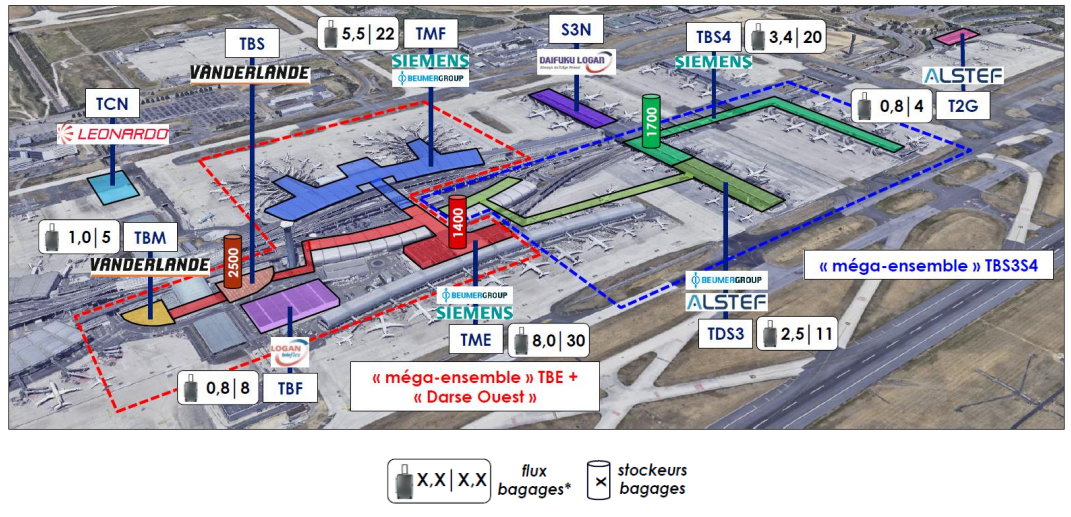
\includegraphics[width=\linewidth]{Plan trieur.png}
    \caption{Map of the different infrastructures}
    \label{fig:Plan trieur}
\end{figure}
\FloatBarrier

Our dataset come from several databases used in the \acrshort{e}. The first called \textit{fact\_paths} contains data of each baggage paths. These data are extracted daily through a pipeline sending requests to the software package used by \acrshort{bhs} managers and analysts. In this table, we access the data of each baggage journey (path) in the \acrshort{bhs}, from the injection of the baggage into the sorter until its extraction.
The second database, \textit{Saria\_info\_vol} contains flight information such as airlines, departure times, departure and destination airports, etc. Thanks to a unique identifier, we are able to link baggage trajectories to information on their inbound and outbound flights. Finally, we could access maintenance data and join some of them to our baggage paths. Those feature not having a significant impact in my models, I won't detail them.\hfill \break

\indent The \autoref{tab:variables} list all data we managed to join. As the aim of this project is to predict the status of baggage when it leaves the \acrshort{bhs}, we need to use data available before it enters the sorter. I spent some time listing and sorting data I could use. I ended up with this list, and decided to use only one data usually available after the sorting process. The path duration (\textit{total\_path\_duration\_no\_stock}) of a bag is known only after the baggage has been sorted. However, as we'll see in the descriptive statistics, path duration is highly correlated with the probability mishandled bags. And as explained in the introduction, Data and management team is currently training some models to predict the duration of bags before it enters the sorter. In \autoref{subsubsec:Paths duration} I explain the methodology to add noise to path duration and therefore transform path duration as a proxy of predicted path duration.

\FloatBarrier
\begin{table}[ht]
    \centering
    \caption{Dictionary of Variables}
    \label{tab:variables}
    \begin{tabularx}{\textwidth}{lclX}
        \toprule
        \textbf{Variable} & \textbf{Type} & \textbf{Description} \\
        \midrule
        id\_bag\_trajet & int64 & Bag path id. \\
        input\_date & datetime & Date and time baggage entered sorter. \\
        input\_module & String & Bag input module. \\
        input\_position & String & Sub-system at which baggage enters sorter. \\
        input\_status & String & Bag status on entering the sorter. \\
        input\_outbnd\_flt\_dhc & Float & Date and time of flight known when bag enters sorter. \\
        output\_module & String & Bag exit module in the sorter. \\
        output\_position & String & Bag exit sub-system. \\
        inbnd\_flt\_hab & datetime &  Date and time of outbound aircraft.\\
        input\_ICT\_BHS & float64 & Time in minutes between baggage injection and the SOBT. \\
        %count\_EBS & int64 & Number of time the bag was stored in \acrshort{ebs} \\
        %count\_TBS & int64 & Number of time the bag was stored in TBS \\
        %has\_flight\_changed & bool & The outbound flight has changed during the bag path. \\
        total\_path\_duration\_no\_stock & float64 & Total baggage transit time in minutes, excluding storage \\
        %path\_length & int64 & Number of times the bag was detected inside the sorter. \\
        %recirc\_gb\_cnt & int64 & Number of additional loop on the primary belt. \\
        %SIBT & datetime & Scheduled inbound time of the intake aircraft. \\
        %AIBT & datetime & Actual inbound time of the intake aircraft. \\
        geographic\_origin & String & Inbound flight origin. \\
        geographic\_dest & String & Outbound flight destination. \\
        SOBT & datetime & Scheduled outbound time of the outbound aircraft. \\
        %AOBT & datetime & Actual outbound time of the outbound aircraft. \\
        30mn\_nb\_bags & int64 & Number of bags entered in the last 30 minutes. \\
        30mn\_nb\_failed & int64 & Number of bags failed in the last 30 minutes. \\
        30mn\_median\_path\_duration & int64 & Median path duration in the last 30 minutes. \\
        nb\_interventions\_needed & int64 & Number of interventions by a human in the last hour across \\ && the TBE \\
        nb\_baggage\_anom & int64 & Number of interventions by a human to correct an issue \\ &&relating to a baggage (stuck or rolling) in the last hour \\ && across the TBE \\
        most\_important\_priority & int64 & Highest priority intervention level in the last hour \\ && across the TBE \\
        is\_failed & bool & Has the baggage been mishandled ? (Variable to predict) \\
        
        \bottomrule
    \end{tabularx}
\end{table}
\FloatBarrier

\newpage
\subsection{Descriptive Statistics}
Every analyses and models in this study were carried out using data from August 1st to October 31st 2023. I decided to analyze these three months, as all the data was available and to have two different types of periods. August is known to have a higher passenger (and therefore baggage) flows, while September and October are quieter months.

\subsubsection{Seasonality}
The sorter opening at around 5 a.m. until 11 p.m. every day of the week, the first intuition we might have about mishandled baggage is the presence of seasonality.
For these reasons, it is important to visualize the evolution of missed baggage over time. \autoref{fig:Average number and percentage of mishandled bags each days of the week}
shows the evolution by day of the week of the number of missed bags, as well as the percentage of
rates

\begin{figure}[h]
    \centering
    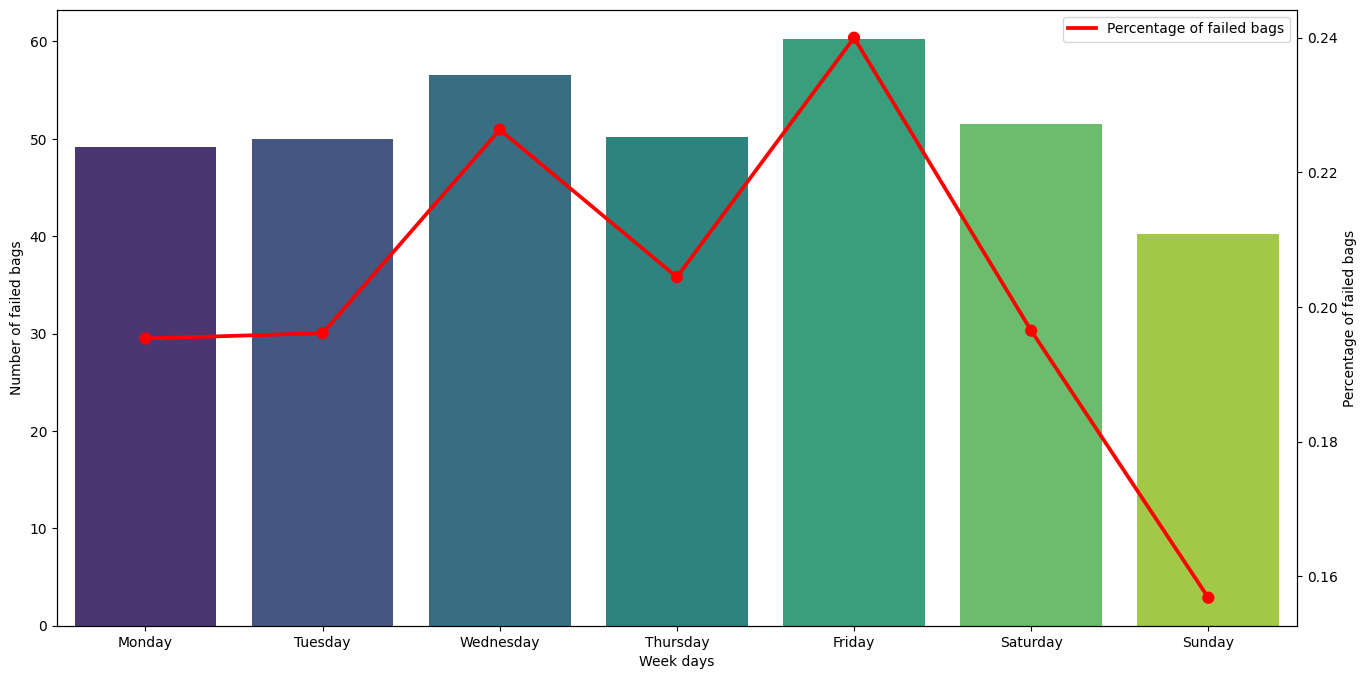
\includegraphics[width=0.9\textwidth]{Number and percentage of failed bags within a week.png}\\
    \caption{Average number and percentage of mishandled bags each days of the week}
    \label{fig:Average number and percentage of mishandled bags each days of the week}
\end{figure}
\FloatBarrier

It's straight forward to see that failed bags volumes are changing according to the week days. Weekends seem to be less problematic, both in terms of volume and percentage. Intuitively, we might have expected weekends to be more complicated (given the greater number of passengers during weekends). Perhaps because logistics teams are more numerous to better manage the heavy flows at weekends, therefore it can be more difficult to avoid failed bags during the week, with teams that could be smaller. Also, as there is a higher number of flights (and thus of bags) during weekends, if the number of mishandled bags remain constant, its percentage will decrease.

To deeper analyse mishandled bags pattern with regard to time, the Figure \ref{fig:Average number and percentage of failed bags each 30 minute of a day} displays the average number and percentage of failed bags for each 30 minute of a day.

\begin{figure}[h]
    \centering
    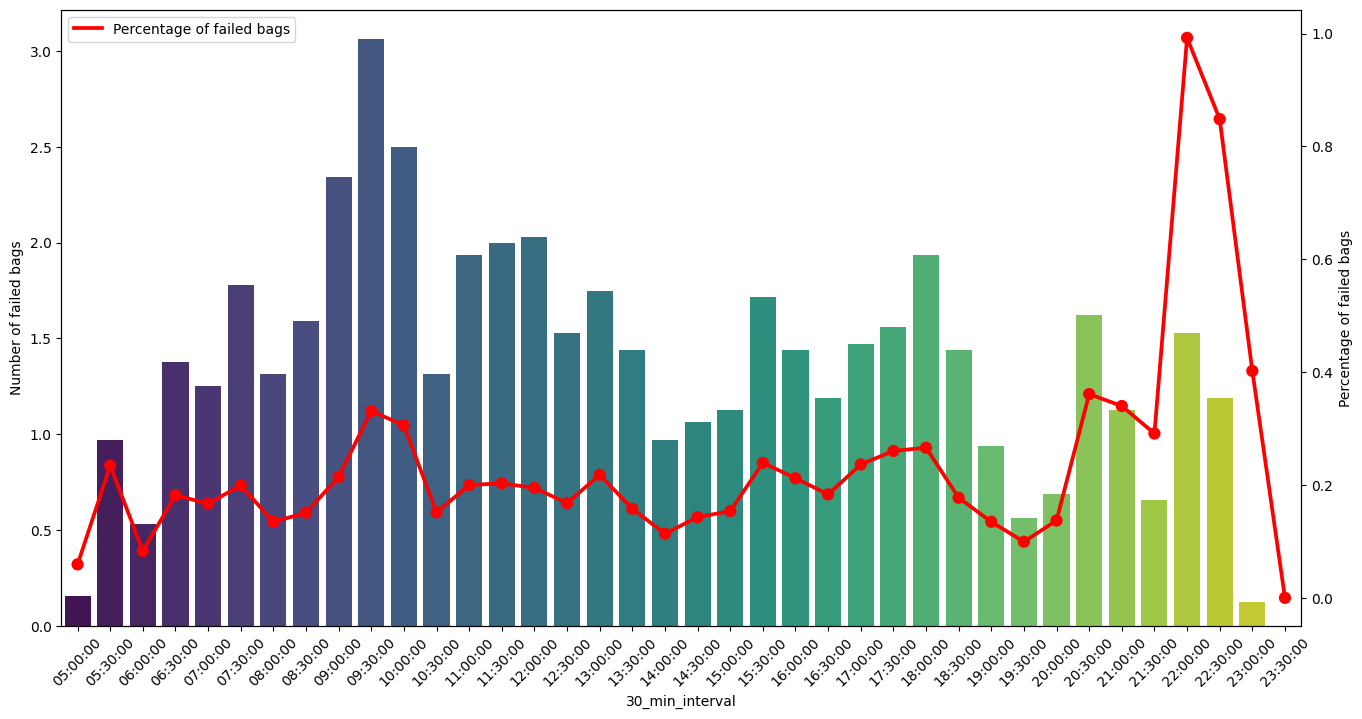
\includegraphics[width=0.9\textwidth]{Number and percentage of failed bags within a day.png}\\
    \caption{Average number and percentage of failed bags each 30 minute of a day}
    \label{fig:Average number and percentage of failed bags each 30 minute of a day}
\end{figure}
\FloatBarrier

It turns out there is a peak of mishandled bags at around 9am in the morning. This could be explained by the large number of flight departure in the morning. We can also see that the percentage of mishandled bags is stable until around 9pm, where it suddenly increase to get its peak. This is most probably due to two reasons. Firstly, handlers feed the sorter at the end of the day with a lot of bags which were mishandled and which will get stored into a store during the night. Those bags are already mishandled before entering the sorter and we have to be aware of this bias while interpreting models results. Moreover, there is less flight at this end of the day, so the number of actual traveling bags is lower while the number of mishandled bags (when being injected) is higher.

\indent Thanks to those figures, we can be sure there are some seasonal effects on the probability to fail a bag. To model it and capture seasonal effects, a special encoding process can be applied as day and hours are cyclical features. Following the method of sin and cosines (\cite{HarrisonPim}) seems to be a great strategy as it encodes minute of the day by taking auto correlation in between minutes that might exist.
\noindent The sinus and cosines transformation are defined as follow : 
\begin{equation}
f(x) = \sin\left(\frac{2\pi x}{\text{period}}\right)
\end{equation}

\begin{equation}
g(x) = \cos\left(\frac{2\pi x}{\text{period}}\right)
\end{equation}

\autoref{fig:Cyclical encoding of days and minutes} displays a visualisation of sin and cosine transformations for a few days only. Each days of the week and minutes of the day are smoothly link to each other, and those smoothed lines (especially for minutes of the days) will help the model to recognize seasonal patterns.  

\FloatBarrier

\newpage
\subsubsection{Baggage paths}

The \acrlong{bhs} being very complex, one of the biggest challenge for \acrshort{adp} in their project to reduce the number of mishandled bags and optimize their logistic is to understand how bags travel inside the \acrshort{bhs}. Using bag paths data, we are able to identify problematic paths, which could be a cause of failed bag. As there is a large number of paths\footnote{There is actually more than 700 different observed paths}, we had to analyse some "typical" or usual paths (paths often used).

To better understand the complexity of the \acrshort{bhs}, I will first explain you how bags travels onto sorter and explain what data I decided to use for bag paths. Then I will provide some statistics about those data.

\paragraph{A journey into the \acrshort{bhs}} Baggage can either come from inbound flights, to be re-routed on inbound flights (i.e. transit baggage), or be injected directly by airlines at check-in counters. Therefore, there are several entry and exit points in the baggage sorting infrastructure.

As showed in \autoref{fig:Plan trieur}, Roissy airport is made up of several \acrlong{bhs}. Siemens and Braumer are the two different manufacturers and technologies that make up the \acrshort{bhs}. At the moment, our team only holds data from the \acrshort{bhs} using Siemens technologies. The \autoref{fig:Simplified diagram of the baggage sorting system "TBE", at the sub-system level} is a simplification of the analysed perimeter (\acrshort{e}). It provides a macro view of the different routes a baggage can take in the sorter.


\begin{figure}[h]
    \includegraphics[width=0.9\textwidth]{synoptique_simplifié.png}\\
    \caption{Simplified diagram of the baggage sorting system TBE, at the sub-system level}
    \label{fig:Simplified diagram of the baggage sorting system "TBE", at the sub-system level}
\end{figure}
\FloatBarrier
Here's a very brief and simplified explanation of a baggage path in the  \acrshort{bhs} : a bag can be injected in the \acrshort{e} by three entrance, the \acrlong{eb1}, the \acrlong{edc}, or by the module F (also called \acrshort{f}). Once a bag enters in the \acrshort{e}, it is routed to \acrshort{etp} in which it will be rerouted (or sorted) to its final destination. If the baggage's flight has not yet been opened, it will be sent to a storage facility (\acrshort{mbis} or \acrshort{ebs}) in which he will wait for his flight to open. If the flight is already open, the baggage will go to the \acrshort{ejt}, where teams of handlers will take it in hand to transport it from the \acrshort{bhs} to the plane.

\paragraph{Simplifiying paths} In fact, baggage paths within the \acrshort{bhs} are far more complex, with many variations. For modeling purposes, I decided to simplify these paths. Instead of taking every check-points of a path, I used only the entry and exit points of each route for two different granularities. The first is the module scale (in which modules the luggage enters and exits), the second is the subsystem scale (in which subsystems the luggage enters and exits). These two granularities provide information on the length and difficulty of the journey, without taking in all the information on the journey. Finally, having more than fifty input positions, and 70 output positions, I first made logical groups of positions. For example, to inject a bag in \acrshort{edc}, there are several different positions. Geographically, these positions are all located in the same hangar, and for handlers, all of these positions are in the the same work warehouse. Therefore, it makes sense to reduce the amount of information by grouping input and output positions by subsystem. In the end, we have five input positions and the three main output positions. 

\FloatBarrier
\begin{figure}[ht]
  \centering
  \begin{subfigure}{0.45\textwidth}
    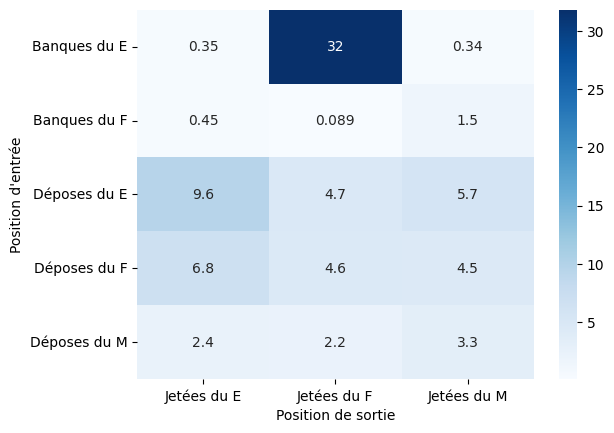
\includegraphics[width=\linewidth]{percentage of failed per positions.png}
    \caption{Percentage of mishandled bags according to input and output positions}
    \label{fig:Percentage of mishandled bags according to input and output positions}
  \end{subfigure}
  \hfill
  \begin{subfigure}{0.48\textwidth}
    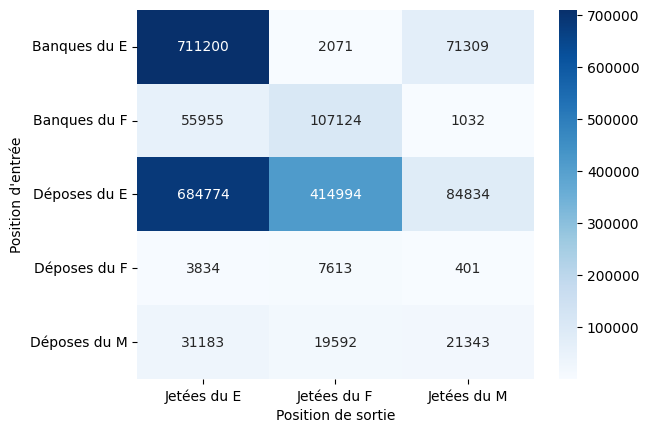
\includegraphics[width=\linewidth]{number of bags per positions.png}
    \caption{Number of bags according to input and output positions}
    \label{fig:Number of bags according to input and output positions}
  \end{subfigure}
  \caption{Mishandled bags according to positions}
  \label{fig:Mishandled bags according to positions}
\end{figure}

\indent The \autoref{fig:Percentage of mishandled bags according to input and output positions} allows us to identify the routes for which we have the highest percentage of mishandled baggage. 
Of all the baggage entering by module banks E (\textit{Banques du E}), and exiting at \acrshort{ejt} (\textit{Jetées du E}), 0.35\% are mishandled. This ratio is very low, especially when compared with the volume of baggage involved in this route, as shown in the \autoref{fig:Number of bags according to input and output positions}. In fact, this route is the most popular. 
However, 9.6\% of bags entering by \acrshort{edc} (\textit{Déposes du E}) and exiting by \acrshort{ejt} (\textit{Jetées du E}) are mishandled, aleven thought this route is also very important in terms of volume. Overall, these two heatmaps allow us to observe the impact of paths from a macro point of view on the probability of a bag being missed.\\
\indent The same analysis were made with the platforms instead of positions. The \autoref{fig:Mishandled bags according to modules} displays the number of bags and the difference in percentage of mishandlded bagages according to which modules it enters and exit. Even though there is less variance in the matrix, modules input and output data will be use to train models.


\subsubsection{Paths duration}\label{subsubsec:Paths duration}

Path duration correspond to the time a baggage spends in the sorter, between entry and exit. In other words, it's the time it takes for ADP's infrastructure to sort and transport a baggage to its destination. These times are very important, because obviously, a baggage spending too much time in the sorter, for whatever reason, could arrive late and miss its flight. They can be seen as indicators of the quality of a baggage's journey through the sorter. 
The \autoref{fig:Distribution of paths duration for non-failed and failed bags} compares the distribution of path duration according to whether they are successful or unsuccessful (mishandled). We can see that mishandled runs have on average much higher times than successful runs (over 20 minutes for unsuccessful runs versus 6 minutes for successful runs).



\begin{figure}[h]
    \centering
    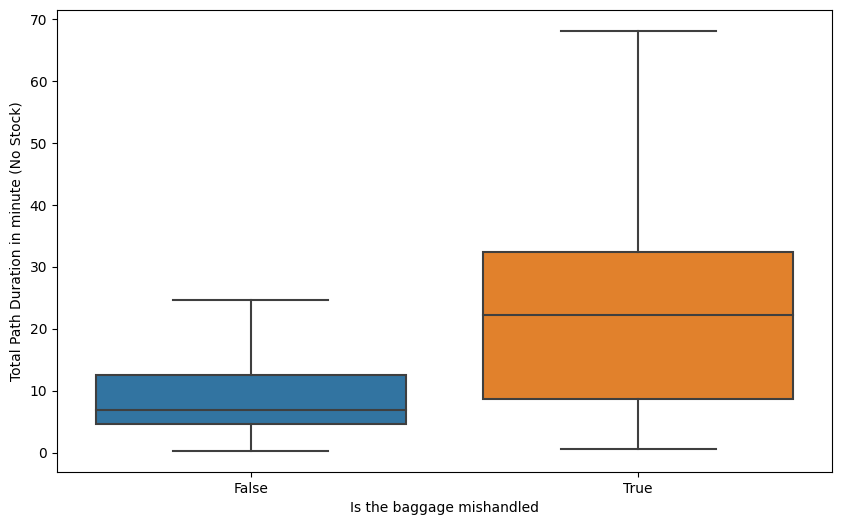
\includegraphics[width=0.6\textwidth]{Boxplot path duration per failed status.png}\\
    \caption{Distribution of paths duration for non-failed and failed bags (without outliers)}
    \label{fig:Distribution of paths duration for non-failed and failed bags}
\end{figure}
\FloatBarrier

For these reasons, travel times can provide a great deal of information for the models, and including them could considerably improve predictions. However, as explained before, we aim to perform our classification at the moment the baggage enters the BHS. The travel time is therefore not yet known at this point. 
To overcome this problem, two methods have been developed.

\paragraph{Past duration time as an indicator} First, the variable \textit{past median duration time} has been created. This corresponds to the median path duration of those who finished their path in the 30 minutes before the baggage to be predicted entered the BHS. This variable could provide the model with information on the quality of baggage handling over the last half-hour.


\paragraph{Using model residuals to generate noise} Secondly, I drew on a modeling project carried out by my colleague Miracle VODOUMBO. He is developing a model for predicting path duration in the \acrshort{bhs}. My idea was to use his predicted travel times to include them as a feature in my prediction model. As Mr. VODOUMBO's model is not yet finished, I decided to use his current residuals to generate noise in the actual travel times. With this method, I add bias to the actual travel times so that they constitute a variable similar to the one that could be predicted in the future. \hfill \break

In order to reproduce the prediction errors as closely as possible, we split the residuals into several groups of travel time quantiles. Indeed, depending on the journey time, the prediction will be more or less accurate. The \autoref{tab:Path duration quantiles} shows the quantile of the travel times used to generate the residuals.


\begin{table}[h]
  \centering
  \caption{Path duration quantiles}
  \label{tab:Path duration quantiles}
  \begin{tabular}{|c|c|c|}
        \toprule
        \textbf{Quantiles} & \textbf{Path Duration (in minute)}  \\
        \midrule
        Q1 & 4.4  \\
        Q3 & 17  \\
        D9 & 28.4  \\
        P99 & 53.3  \\
        \bottomrule
  \end{tabular}
\end{table}  


For each quantile, I have analyzed the residuals of the travel time predictions. The \autoref{fig:Distribution of residuals for path duration between Q1 and Q3} shows the distribution of residuals for runs with a time between Q1 and Q3. Finally, the \autoref{fig:Scatter plot of residuals Vs. path duration (Q1 < time duration < Q3)} shows these same residuals crossed with path duration. It can be seen that the residuals are highly dependent on travel times, and that it is important to generate the residuals correctly so as not to bias path duration too much.

\FloatBarrier
\begin{figure}[ht]
  \centering
  \begin{subfigure}{0.48\textwidth}
    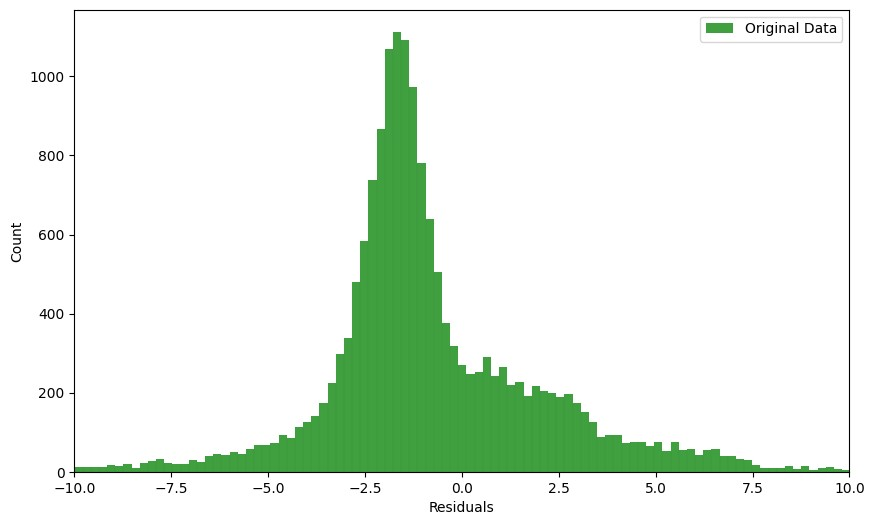
\includegraphics[width=\linewidth]{Q1_Q3 distribution.jpg}
    \caption{Distribution of residuals}
    \label{fig:Distribution of residuals for path duration between Q1 and Q3}
  \end{subfigure}
  \hfill
  \begin{subfigure}{0.48\textwidth}
    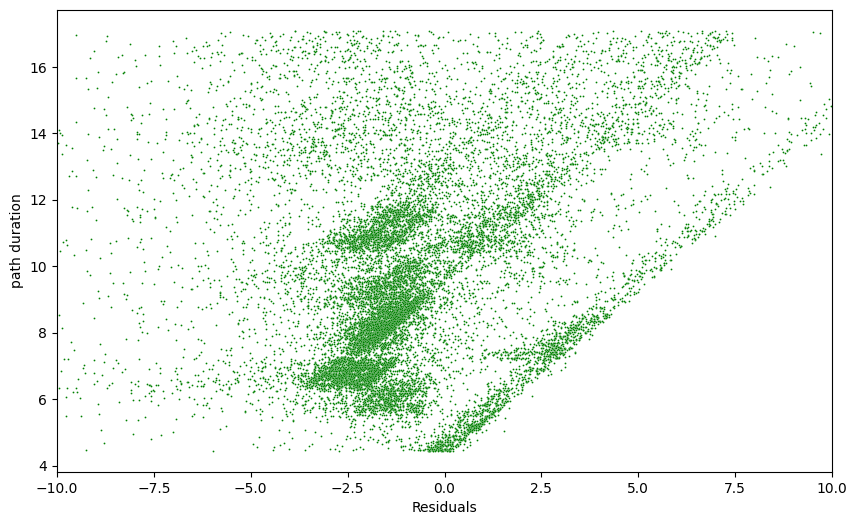
\includegraphics[width=\linewidth]{Q1_Q3 residuals path duration.png}
    \caption{Scatter plot of residuals Vs. path duration}
    \label{fig:Scatter plot of residuals Vs. path duration (Q1 < time duration < Q3)}
  \end{subfigure}
  \caption{Distribution and scatter-plot of residuals for path duration between $Q1$ and $Q3$}
  \label{fig:Distribution and scatter-plot of residuals for path duration between $Q1$ and $Q3$}
\end{figure}

For each different quantile group, I processed a kernel density estimation (see \cite{EMParzen}) which is defined by the function : 
\begin{equation}
f(x) = \frac{1}{nh} \sum_{i=1}^{n} K\left(\frac{x - x_i}{h}\right)
\end{equation}
where : 
\begin{itemize}
    \item \( f(x) \) is the estimated probability density function at point \( x \).
    \item \( n \) is the number of data points.
    \item \( h \) is the bandwidth, a smoothing parameter that determines the width of the kernel function \( K \). \( h \) controls the smoothness of the resulting density function. A small \( h \) can make the estimate too sensitive to small variations in the data (resulting in an estimate with strong noise), while a large \( h\) can over smooth the data, leading to small variance and large bias.
    \item  \( K \) is the Gaussian kernel function, which is a symmetric, non-negative function that integrates to one. We can also swap this function with the Epanechnikov, uniform and many others.
    \item \( x_i \) are the data observed from the sample.
\end{itemize}



The summation \( \sum_{i=1}^{n} \) runs over all the data points, and the function \( K\left(.\right)\) gives the contribution of each data point to the estimation of the density at point \( x \). 


Once done, I generated data from this estimated kernel density. Then, for each of the actual path duration, I searched for the nearest generated path duration (with a binary search algorithm) and assigned its associated generated residual. Under these conditions, there are duplicates in the generated residuals attributed to real travel times. As we can see in the \autoref{fig:Actual Vs. generated residuals (Q1 < time duration < Q3)}, we have more actual than generated data because the only generated data displayed are those assigned to a real travel time. However, the residuals generated are well dispersed and fit well to the residuals of the predictive model. 
\FloatBarrier
\begin{figure}[ht]
\begin{subfigure}[h]{0.5\linewidth}
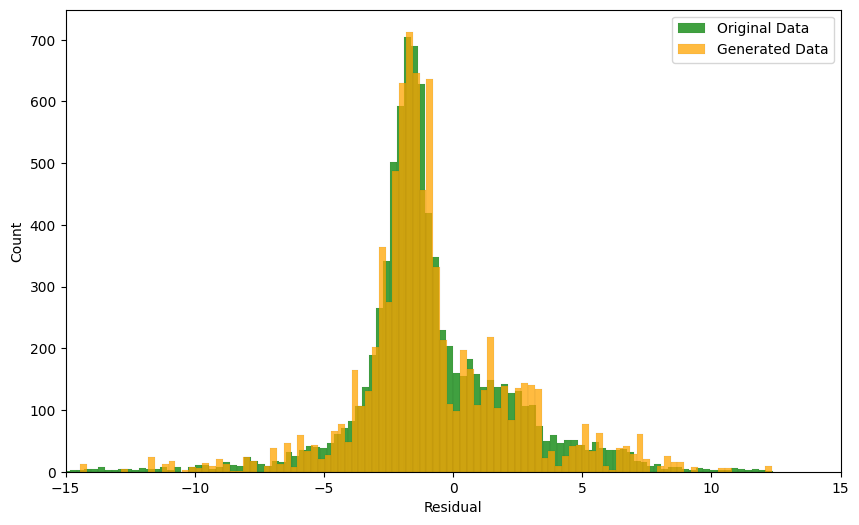
\includegraphics[width=\linewidth]{Q1_Q3 distribution actual Vs. generated.png}
    \caption{Distribution of actual Vs. generated residuals}
    \label{fig:Q1_Q3 distribution actual Vs. generated}
\end{subfigure}
\hfill
\begin{subfigure}[h]{0.5\linewidth}
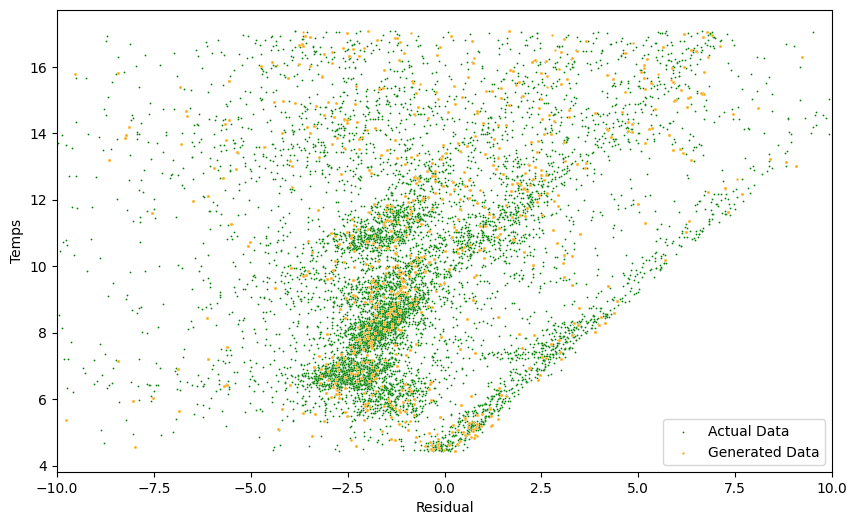
\includegraphics[width=\linewidth]{Q1_Q3 actual Vs. generated.png}\\
    \caption{Actual Vs. generated residuals}
    \label{fig:Actual Vs. generated residuals (Q1 < time duration < Q3)}
\end{subfigure}%
\caption{Comparison of actual and generated data for path duration between $Q1$ and $Q3$}
\end{figure}


Once the residuals have been generated, I had to add them to the actual path duration. However, some of our residuals are negative, so adding them together could result in negative path duration, which makes no sense. To avoid this, the residuals are added only if they are less than the path duration. If this is not the case, then the absolute value of the residual is added. This makes it possible to add residuals without creating negative running times. We can see the comparison of journey times with noise, compared with their actual times in the \autoref{fig:Q1_Q3 path duration noised.png}. The blue curve represents actual path duration, ranked from shortest to longest. The red curve shows the same path duration when the residuals have been added. As can be seen, path duration and residuals are correlated, which was be expected since it's harder for the forecasting model to predict long times than short ones, and the margin of error is also higher.

\FloatBarrier
\begin{figure}[h]
    \centering
    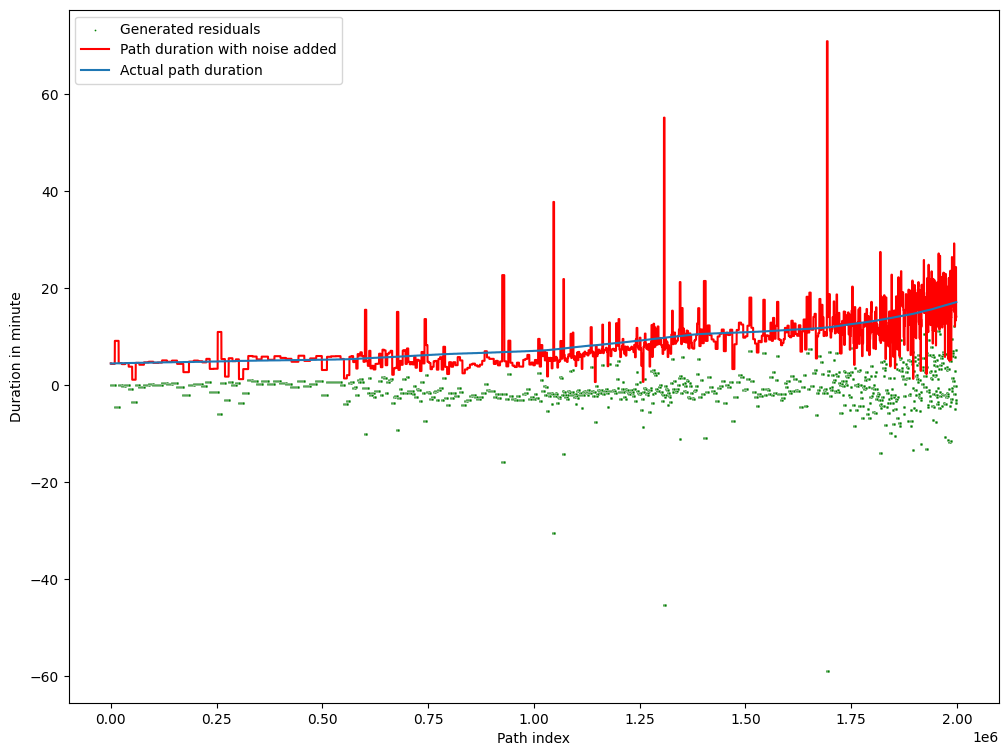
\includegraphics[width=0.8\textwidth]{Q1_Q3 path duration noised.png}\\
    \caption{Comparison of actual path duration with path duration with noise added (Q1 $<$ Path duration $<$ Q3)}
    \label{fig:Q1_Q3 path duration noised.png}
\end{figure}
\FloatBarrier

To conclude, I used the forecasting model of path duration to generate noise and add them up to the actual path duration. This strategy allows me to use the path duration, assuming our department will be able to forecast them before the baggage enters in the \acrshort{e}.

\newpage
\subsubsection{Bags input status}
When being injected onto the sorter, bags are classified according to their status. There exists a lot of status, those indicate how the bag should be sorted. Those status are important and can give information to models.
\begin{figure}[h]
    \centering    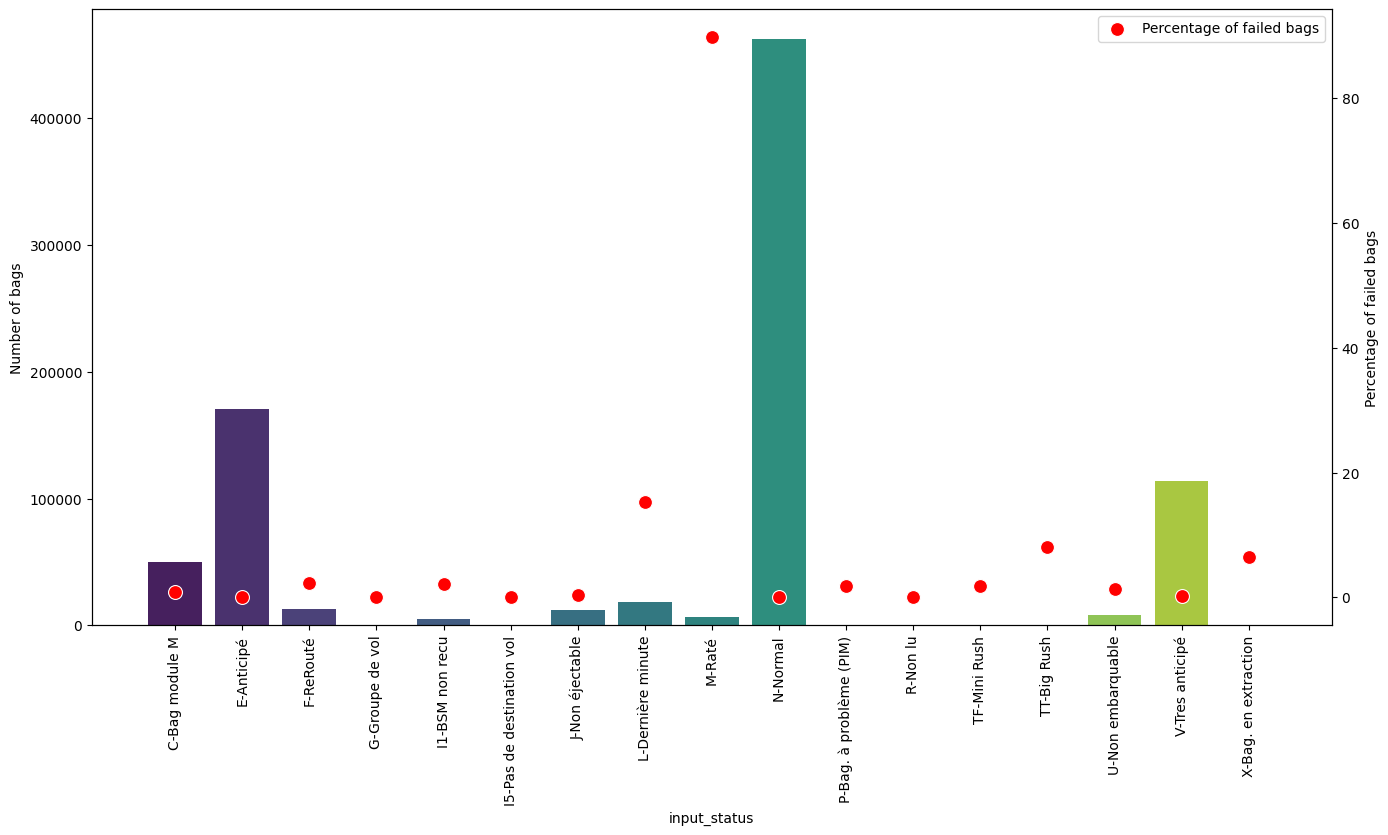
\includegraphics[width=0.8\textwidth]{failed bags per input status.png}\\
    \caption{Number and percentage of failed bags per input status}
    \label{fig:Number and percentage of failed bags per input status}
\end{figure}
\FloatBarrier

All status having different meanings, they also have different frequency. The \textit{normal} status is the most often used and has a low percentage of failed bags. Bags having this status are usually those injected on time in the sorter, when the outbound flight is open to load bags. When a bag is injected earlier and the outbound flight isn't open to load bags, they take the \textit{anticipated} or \textit{very anticipated} status. We could think that injecting a bag much before loading time would be correlated with a lower percentage rate of failed bags. But the \autoref{fig:Number and percentage of failed bags per input status} shows a higher percentage of failed bags for \textit{V-Très anticipé} (very anticipated) bags than \textit{N-Normal} ones. This can be explained by the re-rooting of failed bags. If a flight ends its bag loading process while a bag is still in the sorter, this bag's flight will change (\textit{has\_flight\_changed} will turn \textbf{True}) then its status will change to \textit{V-Très anticipé} (as its unlikely to find another flight soon after missing the previous one) and the bag will be store in a stock to wait.
\noindent The \textit{L-Dernière minute} (last minute) status is given to a bag entering the \acrshort{bhs} knowing there is not much time left. If it manages to exit the \acrshort{bhs} on time, it will be loaded onto the flight with the last minute procedure (manually instead of being put into a container). This status is a very important information for the model as we can see it the category with the higher failed rate (out of \textit{M-Raté}).
\noindent In the aim to model bags output status (failed or not failed), we should carefully consider those \textit{input status} because some of them could make the models to over-fit. For example, \textit{M-Raté} means that the bag is failed when it enters in the \acrshort{bhs}. We should get rid off those kind of bags. 


Finally, here is the list of \textit{input status} we will keep to train and test models : \textit{C-Bag module M, L-Dernière minute, U-Non embarquable, V-Très anticipé, E-Anticipé, P-Bag. à problème (PIM), F-ReRouté, R-Non lu, J-Non éjectable}.


\newpage
\subsubsection{Minute until flight departure}

Another very important data available is the number of minute before flight departure (\textit{input\_ICT\_BHS}). Knowing the \textit{SOBT} of a flight and the \textit{input\_date} of a bag, we computed the number of minute in between both. Looking at the \autoref{fig:Minute until flight departure distribution}, it turns out in average, a bag has a bit less than 200 minutes to reach its flight. The distribution looks to be a gaussian distribution, with some extreme value higher than 600 minutes (\textit{V-Très anticipé} bags) and some negative values. Having a negative number of minute until flight departure mostly mean it's almost impossible to reach its flight on time. However, looking at both distributions of minute until flight departure of mishandled and successful bags in the \autoref{fig:Minute until flight departure distribution according to bag status}, we can see a decreasing proportion of successful bags from approximately 0 to -100 minutes. It means some bags are still managed even when being pushed onto the \acrshort{bhs} after the schedule outbound time. This is most likely explained by flights delays. Those visualisations give us a first important cause of mishandled bags, being injected too late in the \acrshort{bhs}.

\begin{figure}[h]
    \centering
    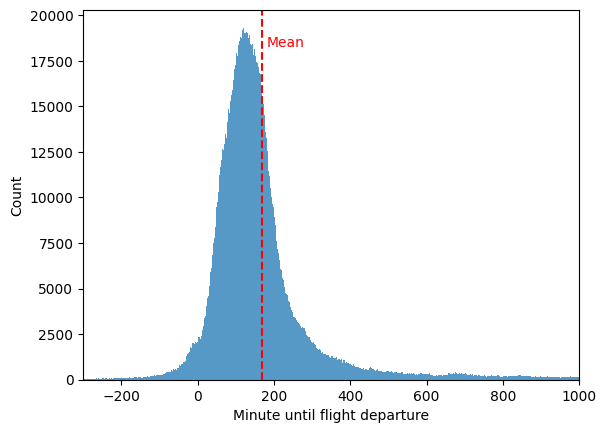
\includegraphics[width=0.6\textwidth]{Minute until flight departure.png}\\
    \caption{Minute until flight departure distribution}
    \label{fig:Minute until flight departure distribution}
\end{figure}
\FloatBarrier

\FloatBarrier
\begin{figure}[ht]
  \centering
  \begin{subfigure}{0.48\textwidth}
    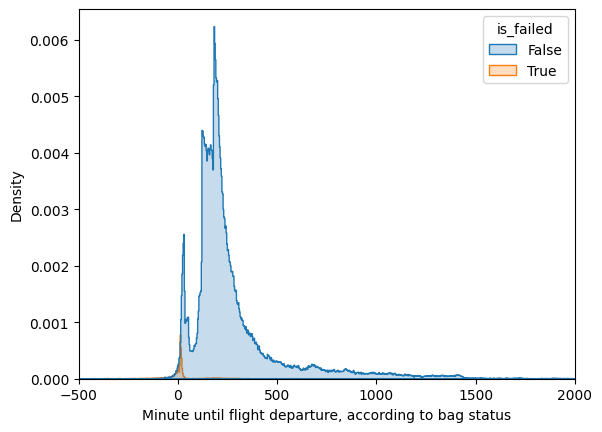
\includegraphics[width=\linewidth]{Minute until flight departure_2.png}
    \caption{Macro view}
  \end{subfigure}
  \hfill
  \begin{subfigure}{0.48\textwidth}
    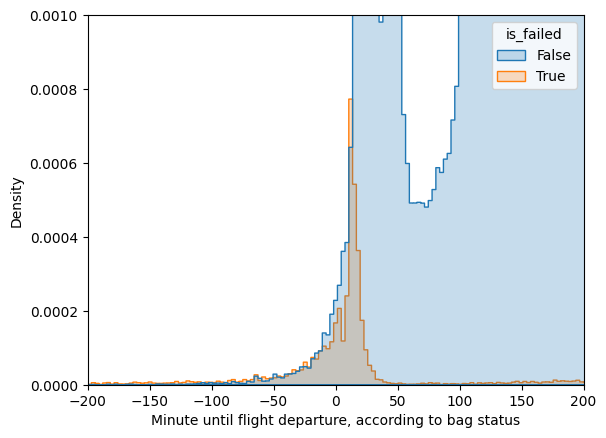
\includegraphics[width=\linewidth]{Minute until flight departure_3.png}
    \caption{Micro view}
  \end{subfigure}
  \caption{Minute until flight departure distribution according to bag status}
  \label{fig:Minute until flight departure distribution according to bag status}
\end{figure}

\newpage
\subsubsection{Geographical links}

Pretty late during the year, I accessed the flights informations of each bag paths data. This dataset concerns only transiting bags\footnote{Bags arriving at CDG airport by an inbound flight in the aim to be loaded in an outbound fight with another destination. Those bags doesn't exit at CDG and are pushed in the \acrshort{bhs} at their arrival.}. It gave us additional informations, and the most relevant were geographical origins and destinations. They are key information in the logistic process for two reasons. 
\begin{itemize}
    \item \textit{Ball baggage} : One of the baggage hazards that can delay a bag journey in the \acrshort{bhs} process is when bag falls off a conveyor belt. When this happens, a handler is called in and has to walk to the location to put the baggage back on the conveyor belt. The handlers have noted that the concerned type of baggage are very often ball baggage, which as the name suggests, are baggage in the shape of a ball (or rounded bags). Because of this shape, they are more likely to roll and fall off the facilities. Finally, although we don't have any statistics on this type of baggage, handlers have pointed out that more often, the origin or destination of the ball bags are African country. For these reasons, including the origin and destination of a baggage can make it possible to include an additional difficulty linked to the type of baggage.


    \item \textit{Parking areas} : The second impact of origin and destination is the flight parking areas. As flight companies share terminal and check in doors, they also share parking areas. We don't have exact plans of it, but as the airport is extremely large, the destination and origins of flights could add geographical information within the airport in the model. For example, if a bag comes from an european country and is going to another european country, it is more likely that it uses the same company for both flights. Therefore, the path and process in between its arrival and departure would be shorter. On the other hand, a bag coming from Ireland and taking a flight for China will probably not use the same company. So the parking areas might be more far away from each other.
\end{itemize}


For the locations, even though we had precised data like name of airports and countries, I decided to use continent only to reduce the complexity of models and avoid unnecessary noise. 

\noindent To encode those data, I grouped each possible origins and destinations links possible. As we are interested by the links effect (for example a bag from Africa and going to America), it would be more efficient for models to have one column for links (\textit{from Africa to America}) instead of two separated columns for origin and destination. Finally, as those are categorical data I encoded them with the one-hot encoder strategy.

\newpage
\section{Imbalanced dataset issue}\label{section:Imbalanced dataset issue}

The question of unbalanced datasets is one of the interesting issues to deal with in machine learning. In a classification, we want to predict which of the different possible events will occur. To train an algorithm, it needs a certain amount of data in order to calibrate its coefficients with the training dataset, and test the best theoretical coefficients with the test dataset. During classification, the different classes may not be equally distributed.

\begin{figure}[htbp]
    \centering
    \begin{minipage}{0.55\textwidth}
        \centering
        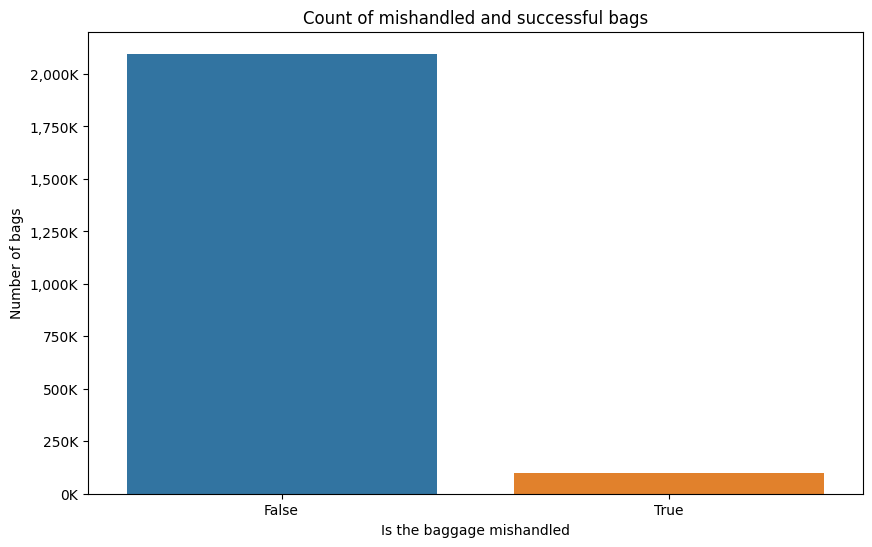
\includegraphics[width=\textwidth]{is_failed unbalanced.png} % Replace 'example-image' with your image file
        \caption{Proportion difference of mishandled and successful bag}
        \label{fig:Proportion difference of failed and non-failed bag}
    \end{minipage}
    \hfill
    \begin{minipage}{0.3\textwidth}
        In our case of mishandled baggage, the \autoref{fig:Proportion difference of failed and non-failed bag} shows the difference between the number of successful and mishandled bags. Fortunately for passengers, the number of mishandled bags is far smaller than the number of successful bags. In our dataset, there are 2 mishandled bags for every 100 successful bags.
    \end{minipage}
\end{figure}

This large difference in proportions is problematic, because when training the models, there's a risk of over-training them to predict successful baggage (see \cite{ArtificialIntelligenceReview}).Indeed, if 98\% of baggage are not mishandled, the models will be able to get a good score by predicting 100\% of successful baggage. However, there is a risk of not being able to predict missed baggage. To overcome this problem, we first take a look at the confusion matrix. Having a look at the \autoref{tab:Confusion Matrix}, we can try to understand the confusion matrix concept. 
\begin{table}[htbp]
    \centering
    \captionsetup{justification=centering}
    \caption{Confusion Matrix}
    \label{tab:Confusion Matrix}
    \newcommand{\cellcolorpos}{\cellcolor{cyan!20}}
    \newcommand{\cellcolorneg}{\cellcolor{yellow!20}}
    \begin{tabular}{cc|c|c|}
        \cline{3-4}
        & & \multicolumn{2}{c|}{\textbf{Actual}} \\
        \cline{3-4}
        & & \textbf{Positive} & \textbf{Negative} \\
        \hline
        \multicolumn{1}{|c|}{\multirow{2}{*}{\textbf{Predicted}}}
        & \textbf{Positive} & \cellcolorpos True Positive (TP) & \cellcolorneg False Positive (FP) \\
        \cline{2-4}
        \multicolumn{1}{|c|}{}
        & \textbf{Negative} & \cellcolorneg False Negative (FN) & \cellcolorpos True Negative (TN) \\
        \hline
    \end{tabular}
\end{table}
\noindent This matrix gives four different informations : 
\begin{itemize}
\centering
    \item \acrshort{tp} : The model predicted a \textit{True} event while it was actually \textit{True}.
    \item \acrshort{tn} : The model predicted a \textit{False} event while it was actually \textit{False}.
    \item \acrshort{fp} : The model predicted a \textit{False} event while it was actually \textit{True}.
    \item \acrshort{fn} : The model predicted a \textit{True} event while it was actually \textit{False}.
\end{itemize}

Therefore in the context of mishandled baggage issue, we might manage to predict a high number of successful bags (FP will be high) but struggle to predict mishandled bags as it is the minority class (TP will be lower). 
Having a look at some metrics might help to understand the problem and how to manage it.
The accuracy compute the ratio of good predictions over all the population. It doesn't mind if one of the class got a bad prediction score. Using this metric only can lead to over estimate the capacity of the model. If the model predict 100\% of the bags as successful, as it is the majority class, the accuracy might be very high even though the number of TP is null. 
\begin{equation}
\text{Accuracy} = \frac{\sum{TP + TN}}{\sum{TP + TN + FP + FN}}    
\end{equation}

The recall compute the ratio of TP over the TP and the FN populations. Having a high recall rate means we didn't predict much actually positive status as negative one. In the bags issue, it means we would not predict mishandled bags as successful. Reversely, having a low recall means we predict too much mishandled bags as being successful. This ratio will be very important as it will give information on the ability of the model to predict mishandled bags.
\begin{equation}\label{equation:Recall}
\text{Recall} = \frac{\sum{TP}}{\sum{TP + FN}}    
\end{equation}

The precision is the ratio of TP over TP and FP populations. It measures how many of the predicted positive instances are actually positive. A high precision indicates that when the model predicts positive values, it is actually correct (So we have a lower number of FP).

\begin{equation}\label{equation:Precision}
\text{Precision} = \frac{\sum{TP}}{\sum{TP + FP}}
\end{equation}

\noindent Both recall and precision are important to optimise a model, especially when to target classes are imbalanced. However, deciding to optimise the recall to predict the maximum of mishandled-bags would also increase the number of false positive (successful bags predicted as mishandled). Reversely, optimising the model by maximising the precision would increase the false negative, meaning that more mishandled bags wont be predicted. 
To find the best trade-off between precision and recall, the F1-score combines both metrics. A high F1-score coefficient indicates that both recall and precision are quite good. In such a case, we can consider the model as accurate for positive predictions. In the case of imbalanced dataset, the F1-score will give more balanced measured by considering both precision and recall. 
\begin{equation}\label{equation:F1-score}
\text{F1-Score} = 2 \cdot \frac{\text{Precision} \cdot \text{Recall}}{\text{Precision} + \text{Recall}}    
\end{equation}







\newpage
\section{Models}
Before turning to the methodology and results, this section will present the machine learning algorithms and methods used.\hfill \break
\indent I decided to use three different algorithm.
The \acrlong{lr} is my benchmark model (as in \cite{MishandledBgas}) and will be use to verify if my other more complex models improve the performance of the predictions. 
Then, I trained and tested two ensemble models\footnote{Ensemble methods use multiple learning algorithms to obtain better predictive performance than could be obtained from any of the constituent learning algorithms alone (definition from \cite{wikiensemble})}. The \acrfull{rf} is often used for classification tasks as it combines the strengths of multiple individual models (decision trees) to improve the classification and avoids randomness of decision trees. It also reduces over fitting and increases generalization of the classification problem.
On the other hand, \acrfull{xgboost}, an evolution of the \acrshort{rf}, enhances performance by sequentially building trees that correct errors from previous one.
Both of those ensemble models car capture complex non-linear patterns and lead to more accurate predictions.
Finally, in the aim to transform scores into probabilities, I used the Platt-Scaling and Isotonic regression methods, both for \acrshort{rf} and \acrshort{xgboost}. Those methods are embedded models. Using a classifier, we can train a calibration model to calibrate its predicted probabilities, such that we can analyse them as probabilities instead of scores (which are more difficult to analyse).


\subsection{Random Forest}\label{subsec:Random forest}
 
Introduced by \cite{Breiman2001}, \acrlong{rf} operates by constructing a multitude of decision trees (\cite{DecisionTrees}) during training and outputting the class that is the mode of the classes\footnote{classification} or mean prediction\footnote{regression} of the individual trees. 

When building a decision tree, at each node a sub sample is selected randomly among the entire subset (see \cite{LouppeRF}). Therefore, using a decision tree as a predictive model is likely to be non-efficient and under-fit as the parameters will depends on the sub-sample drawn. The \acrshort{rf} algorithm was developed as an extension of decision trees. By constructing a multitude of decision trees and averaging the predicted labels (or continuous predictions) avoids the main decision tree issue. This method is known as bagging\footnote{as well as bootstrap sampling} and makes \acrshort{rf} be part of the ensemble models family.\hfill \break

The Random Forest algorithm can be summarized in the following steps:
 
\begin{enumerate}
    \item Draw $n$ bootstrap samples from the original dataset.
    \item For each bootstrap sample, grow decision tree. At each node, randomly select $m$ features from the total $p$ features. \item Choose the best feature among the $m$ to split the node.
    \item Repeat steps 1, 2 and 3 for a predefined number of trees.
    \item Aggregate the predictions of the trees (by majority voting for classification or averaging for regression).
\end{enumerate}



\begin{algorithm}[H]
\caption{Random Forest Algorithm}
\begin{algorithmic}
\STATE \textbf{Input:} Training data $(x_i, y_i)$, number of trees $N$, number of features $m$
\STATE \textbf{Initialize:} $f_0(x)$
\FOR{$i = 1$ to $N$}
    \STATE Draw a bootstrap sample $D_i$ from the training data
    \STATE Grow a decision tree $T_i$ on $D_i$:
    \FOR{each node in $T_i$}
        \STATE Randomly select $m$ features from $p$
        \STATE Choose the best feature among the $m$ to split the node
    \ENDFOR
\ENDFOR
\STATE \textbf{Output:} Aggregate the predictions of $N$ trees
\end{algorithmic}
\end{algorithm}
 
%\acrlong{rf} can be seen as optimizing the following objective function for classification :
 
%\begin{equation}\label{equa:Objective function for Random Forest}
%L(f) = \sum_{i=1}^n L(y_i, \hat{y}_i)
%\end{equation}
 
%where $L(y_i, \hat{y}_i)$ is the loss function, which is the following logistic loss for classification :

%\begin{equation}\label{equa:Log Loss function}
%L(f) = \sum_{i=1}^n L(y_i, \hat{y}_i)
%\end{equation}
 

The \acrshort{rf} model even if more interpretable than models like \acrshort{xgboost}, still can be seen as a black box\footnote{Model whose internal logic and decision-making process are not easily interpretable by humans. While the model inputs and outputs are known, the inner logic that transform the inputs onto outputs is opaque.} when considering the entire forest. However, I decided to use it for its robustness and effectiveness in various predictive tasks.


\subsection{Extreme gradient boosting}
\label{subsec:Extreme Gradient Boosting}

The \acrlong{xgboost}, introduced by \cite{https://arxiv.org/pdf/1603.02754}, is a machine learning algorithm popular for its efficiency. It was designed as an extension\footnote{Gradient boosting is a machine learning technique used for regression and classification tasks. It builds models in a sequential manner, where each new model corrects errors made by the previous ones. By combining these models, it creates a final strong model that improves prediction accuracy. (\cite{Friedman2001})} of the \acrshort{rf} such that it can handle large and complicated dataset. In our complex mishandled bags issue, it essential to train and optimise such a model to compare its results to the others (especially to the Logistic regression and the Random Forest).

Unlike \acrshort{rf} which is a bagging gradient method, the XGBoost uses gradient boosting approach where trees are built sequentially to correct and adjust the error of previous trees. It is this main important difference that enables XGBoost to achieve more accurate results than \acrshort{rf}. The XGBoost algorithm is a pretty efficient and speed one for large dataset, as it utilize advanced optimization techniques such as parallel processing and cache awareness. Moreover, including both L1 (Lasso) and L2 (Ridge) regularization techniques, XGBoost also prevent over-fitting and increase the generalization\footnote{Adaptation ability of the model with new and unseen data} power. \hfill \break


Following and retracing the literature of the \cite{IntroductionToBoostedTrees}, the algorithm can be summarized in the following steps:
 
\begin{enumerate}
    \item Initialize the model with a base prediction, usually the mean of the target values. 
    \item For a predefined number of iterations:
    \begin{enumerate}
        \item Compute the gradient of the loss function with respect to the current model's predictions.
        \item Fit a decision tree to the residuals.
        \item Update the model by adding the fitted tree, scaled by a learning rate.
    \end{enumerate}
    \item The final model is the sum of the base prediction and all the fitted trees.
\end{enumerate}

\begin{algorithm}[H]
\caption{XGBoost Algorithm}
\begin{algorithmic}
\STATE \textbf{Input:} Training data $(x_i, y_i)$, number of iterations $M$, learning rate $\eta$
\STATE \textbf{Initialize:} $f_0(x) = \log ( \frac{\bar{y}}{1 - \bar{y}})$
\FOR{$m = 1$ to $M$}
    \State Compute the residuals: $r_{im} = -\left[ \frac{\partial L(y_i, f(x_i))}{\partial f(x_i)} \right]_{f(x)=f_{m-1}(x)}$ \hfill \break
    \State Fit a decision tree $h_m(x)$ to the residuals $r_{im}$ \hfill \break
    \State Update the model: $f_m(x) = f_{m-1}(x) + \eta h_m(x)$
\ENDFOR
\STATE \textbf{Output:} Final model $f_M(x) = f_0(x) + \sum_{m=1}^{M} \eta h_m(x)$
\end{algorithmic}
\end{algorithm}
\FloatBarrier



\noindent Diving into the maths, XGBoost algorithm optimizes the following objective function:
 
\begin{equation}\label{equa:Gradient Boosting objective function}
\mathcal{L}(f) = \sum_{i=1}^{n} L(y_i, \hat{y}_i) + \sum_{m=1}^{M} \Omega(h_m) 
\end{equation}
where:
\begin{itemize}
    \item $L(y_i, \hat{y}_i)$ is the logistic loss for classification.
    \item $\Omega(h_m)$ is the regularization term for the $m$-th tree, defined as:
    \begin{equation}
    \Omega(h_m) = \gamma T + \frac{1}{2} \lambda \sum_{j=1}^{T} ||w_j||^2
    \end{equation}
    where we have two regularization parameters. $\gamma$ controls the number of leaves $T$ and $w_j$, the weight of leaf $j$, is penalized by $\lambda$ when it turns too heavy. Both parameters are extremely precious in the aim of generalization.
\end{itemize}


\noindent The gradient boosting framework updates the model by adding the tree that minimizes the following objective:
 
\begin{equation}\mathcal{L}^{(m)} = \sum_{i=1}^{n} \left[ L(y_i, \hat{y}_i^{(m-1)}) + g_i h_m(x_i) + \frac{1}{2} h_i h_m(x_i)^2 \right] + \Omega(h_m)
\end{equation}
 
where $g_i$ and $h_i$ are the first and second-order gradients of the loss function with respect to the predictions:
 
\begin{equation}\label{equa:test}
g_i = \frac{\partial L(y_i, \hat{y}_i^{(m-1)})}{\partial \hat{y}_i^{(m-1)}}, \quad h_i = \frac{\partial^2 L(y_i, \hat{y}_i^{(m-1)})}{\partial \hat{y}_i^{(m-1)2}}    
\end{equation}

 
The tree is then fitted to the negative gradients, and the weights are adjusted to minimize the objective function, incorporating both the loss and the regularization term. \hfill \break



As the XGBoost model is very complex, it is considered a black box in which it is virtually impossible to interpret the coefficients. However, we'll be using it for its accuracy, with the aim of predicting missed baggage as accurately as possible.


\subsection{Probability calibration}
\label{subsec:Probability calibration}

Classifier models used classify data according to predicted scores. However, these scores cannot be interpreted as probabilities.
Indeed, when a model learns and predicts unbalanced data, it is likely to underestimate the probability of events in the minority class. In our case, models are likely to assign too low a probability to missed baggage\footnote{A phenomenon also known as distortion}. For this reason, classifier scores aren't considered as predicted probabilities but scores. 

First introduced by \cite{Zadrozny2002} (and pretty well explained by \cite{ProbabilityCalibration}\footnote{Articles \cite{JasonBrownlee} and \cite{ExperianLatAmDataLab} were also used to understand these concepts}) Platt Scaling and Isotonic regression are both most common method of probability calibrations.

\subsubsection{Platt Scaling}
 
Platt scaling involves fitting a logistic regression model to the classifier scores. The logistic regression model is trained using the classifier scores as input and the true binary labels as the target. In the case of baggage issue, the classifier score are the predicted probability that a baggage is mishandle, and the true binary label is the actual final status of the baggage, being successful or mishandled. The formula for platt scaling is given by :

\begin{equation}
P(y=1|x) = \frac{1}{1 + \exp(Af(x) + B)}    
\end{equation}

where \( f(x) \) is the predicted probability of the classifier for input \( x \), and \( A \) and \( B \) are parameters learned from the training data. Both parameters are estimated using maximum likelihood method. And gradient descent is used to solve:

\begin{equation}
\arg\min_{A,B} \left\{ -\sum_{i} y_i \log(p_i) + (1 - y_i) \log(1 - p_i) \right\},
\end{equation}
where,
\begin{equation}
p_i = \frac{1}{1 + \exp(Af_i + B)}
\end{equation}




\subsubsection{Isotonic Regression}

The isotonic regression is a non-parametric method where the only restriction is that the estimated function should be monotonically increasing (isotonic).
The isotonic regression can be mathematically written as :

\begin{equation}
y_i = m(f_i) + \epsilon_i
\end{equation}
 where $f\_i$ is the classifier score and $y_i$ the true target.
 Then, we find the isotonic function $\hat{m}$ such that :
\begin{equation}
\hat{m} = \arg\min_{z} \sum_{i} \left( y_i - z(f_i) \right)^2
\end{equation}


For both method, using the same training set for the first classifier and the calibration would lead to over-fit. Thus, we need to have a second hand calibration dataset used to train the platt scaling and isotonic regression after having trained the classifier with the main train dataset. 

\newpage
\section{Methodology}
All the machine learning models used were trained using the same methodology, otherwise their results would not be comparable.
This section details the methodology used to train and test the algorithms.

\paragraph{Data normalization} Continuous data normalization is a crucial step in the modeling process. It consists in transforming the scale of the data so that all data are comparable. Without this transformation, algorithms could over-estimate the importance of a feature due to its much larger scale than another feature. Under these conditions, data normalization increases the predictive performance of models, or in other words, reduces its degradation.
As my data contains outliers (which I haven't removed), Robust Scaler is particularly effective as this method is based on the median and interquartile range.\footnote{Library : \cite{RobustScaler}}, which makes it less sensitive to outliers\footnote{In the contrary, Standard Scaler method is based on the mean and standard deviation. As a result, having outliers can bias the scaling and make it less efficient.}. 
This allows the data to be centered and reduced so that extreme values do not disproportionately influence the results, providing a more reliable representation of data characteristics for machine learning algorithms. Bellow is the function used for the robust scaling.

\begin{equation}
x_i = \frac{x_i - Q_1(x)}{Q_3(x) - Q_1(x)}    
\end{equation}
where $Q_1$ is the 1st quartile, and $Q_3$ is the third quartile.


\paragraph{Data splitting} In most training cases, the data is split between a train set and a test set. In my case, I split my data between a train, a test and calibration datasets.
The calibration dataset was used separately to calibrate the data, using the platt scaling and isotonic regression methods (explained in \autoref{subsec:Probability calibration}). The \autoref{fig:Data split} shows how data has been split in proportion.
\begin{figure}[h]
    \centering
    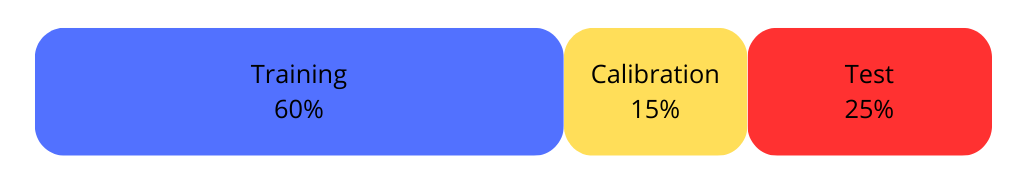
\includegraphics[width=0.9\textwidth]{Data splitting.png}\\
    \caption{Data split}
    \label{fig:Data split}
\end{figure}
\FloatBarrier
This split method was applied for training, calibration and testing by setting the random state. In this way, all algorithms had the same data for each modeling step. 
Finally, each dataset contained the same proportion of failed baggage. By using the function \textit{stratify} of sklearn\footnote{Library : \cite{StratifySplit}}, we can make sure that the minority class will always have the same proportion. If we don't do this, we could end up with, for example, too many failed test sets and too many failed training sets. Under these conditions, our test results would be biased.

\paragraph{Cross validation}
Cross-validation is an essential technique in training, as it enables the performance of a model to be assessed more robustly and reliably. Unlike a simple separation of data into training and test sets, cross-validation divides the data into several subsets or “folds”, then trains and tests the model on different combinations of these subsets. This reduces the risk of bias due to a specific partition of the data, and provides a more accurate estimate of the model's ability to generalize to unseen data. In short, cross-validation helps to avoid over-fitting and ensures that the model is well adapted to predict varied data, making its predictions more reliable in production. Cross-validation is used with the train dataset, which is split into four folds.
\begin{figure}[h]
    \centering
    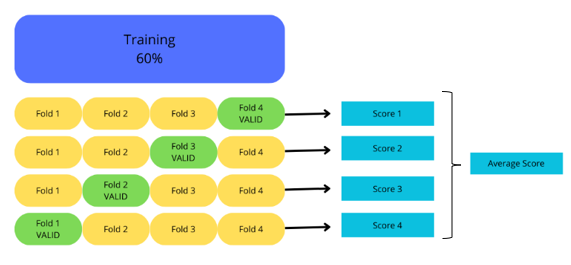
\includegraphics[width=0.85\textwidth]{KFold data.png}\\
    \caption{KFold cross-validation}
    \label{fig:KFold cross-validation}
\end{figure}
\FloatBarrier
The \autoref{fig:KFold cross-validation} shows how the training set has been split for cross-validation. We have four different folds. The models have therefore been trained separately but with the same parameters four times and tested on four different dataframes. Their four scores are then calculated and aggregated into an average, which is the final model score. By using this method, we avoid a model performing better randomly depending on the training or test dataset. 


\paragraph{Hyper parameter optimization}
Machine learning algorithms can contain a large number of parameters, specifying how the learning tasks should process (such as the number or depth of trees). Those are called hate, hyper-parameters. A way to optimize an algorithm is to optimize those parameters. For this purpose, there exists two popular methods. 
The grid search consists in setting a couple of possible values for each parameters, train the algorithm for each possible combination of them, and keep the combination with the highest score.
The random search consists in setting a certain distribution function for each parameters, and draw each combination randomly. With such a method, we can find certain region of parameters where they are more or less efficient. \hfill \break
I firstly used the grid search method to find a first set of parameters, and then tried to improve the score with a random search.\hfill \break

The \autoref{fig:Final sets of hyper-parameters} display the final sets of parameters for both \acrshort{rf} and \acrshort{xgboost}. Those were find with the random search method.

\FloatBarrier
\begin{table}[h!]
    \centering
    \caption{Final sets of hyper-parameters}

    \begin{tabular}{lccc}
        \toprule
        \textbf{Parameter} & \multicolumn{2}{c}{\textbf{Model}} \\
        \cmidrule{2-3}
         & \textbf{\acrshort{rf}} & \textbf{\acrshort{xgboost}} \\
        \midrule
        criterion & Entropy &  \\
        min samples leaf & 1 &  \\
        max depth & 35 & 31 \\
        nb. estimators & 278 & 188 \\
        column sample by tree & & 0.63  \\
        eta & & 0.06  \\
        reg lambda & &0.88 \\
        sub sample && 0.87\\
        min child weight && 1\\
        \bottomrule
    \end{tabular}
    \label{fig:Final sets of hyper-parameters}
\end{table}
\FloatBarrier



\paragraph{Concept of class weights}

\noindent Class weights are coefficients assigned to classes in order to handle imbalanced datasets. When data is imbalanced, the class with the majority of instances can dominate the learning process, causing the model to perform poorly on the minority class. By assigning higher weights to minority classes and lower weights to majority classes, the model can be made more sensitive to the minority class, improving overall performance. For imbalanced datasets, class weights adjust the learning algorithm to pay more attention and give more power to the minority class, helping to balance the model's performance across all classes. \hfill \break
 
In a \acrlong{lr}, class weights are incorporated into the loss function (see \cite{AppliedMachineLearning}). The weighted loss function is then given by :
\begin{equation}
L(\theta) = -\sum_{i=1}^{n} w_i \left[ y_i \log(p_i) + (1 - y_i) \log(1 - p_i) \right]
\end{equation}
 
where \( w_i \) are the class weights, \( y_i \) are the true labels, and \( p_i \) are the predicted probabilities. \hfill \break
 
In \acrlong{rf}, class weights can be applied to the criterion used to split the nodes. The Gini impurity or entropy can be weighted by the class weights. For instance, the weighted Gini impurity is:

\begin{equation}
G_w = \sum_{k=1}^{K} w_k p_k (1 - p_k)
\end{equation}
 
where \( w_k \) is the weight for class \( k \), and \( p_k \) is the proportion of class \( k \) at a given node. \hfill \break
 
For \acrshort{xgboost}, class weights can be used to scale the gradients and Hessians during the boosting process. The weight-adjusted loss function for \acrshort{xgboost} algorithm can be represented as:
 
\begin{equation}
L(\theta) = \sum_{i=1}^{n} w_i \ell(y_i, f(x_i))
\end{equation}
 
where \( \ell \) is the loss function, \( w_i \) are the class weights, \( y_i \) are the true labels, and \( f(x_i) \) are the model predictions.


\paragraph{Classification threshold choice} 
In our binary classification models, the aim is to predict whether a bag will be mishandled. We therefore have a binary output. Instead of directly giving a class as output, the model produces scores. These scores indicate the model's confidence in the bag being successful or mishandled.
 
For example, if the model gives a score of 0.7 and classifies the bag as negative, we can say that it predicts that there is a greater chance that the bag will fail than succeed. By default, the models used classify baggage as mishandled if the score is greater than 0.5 and as successful if the score is less than 0.5. However, this arbitrary classification is not always the one that optimizes the score, especially when dealing with unbalanced data. 
To improve classification, a different threshold can be defined.
Optimizing the F1-score involves finding the threshold that maximizes this metric. 
Thus, I have calculated the F1-Score for all existing thresholds from 0 to 1. Finally, the classification threshold kept is the one for which the F1-Score is the highest.


\paragraph{Providing actual probabilities} As explained in the \autoref{subsec:Probability calibration}, predicted score are not always probabilities. In order to give probabilities instead of predicted scores, we can perform probability calibration. However, this step must be carried out rigorously to avoid over fitting. \hfill \break
Probability calibration isn't done with training data. Firstly, we need to train the models with the train data. Then, the predicted scores are given to the probability calibration models (platt scaling and isotonic regression) to train them.\footnote{This type of method is known as an "embedded model”: a model that contains at least one variable predicted by another model.}. The \autoref{fig:Methodogoly} gives a overview of the entire set-up methodology.

\begin{figure}[h]
    \centering
    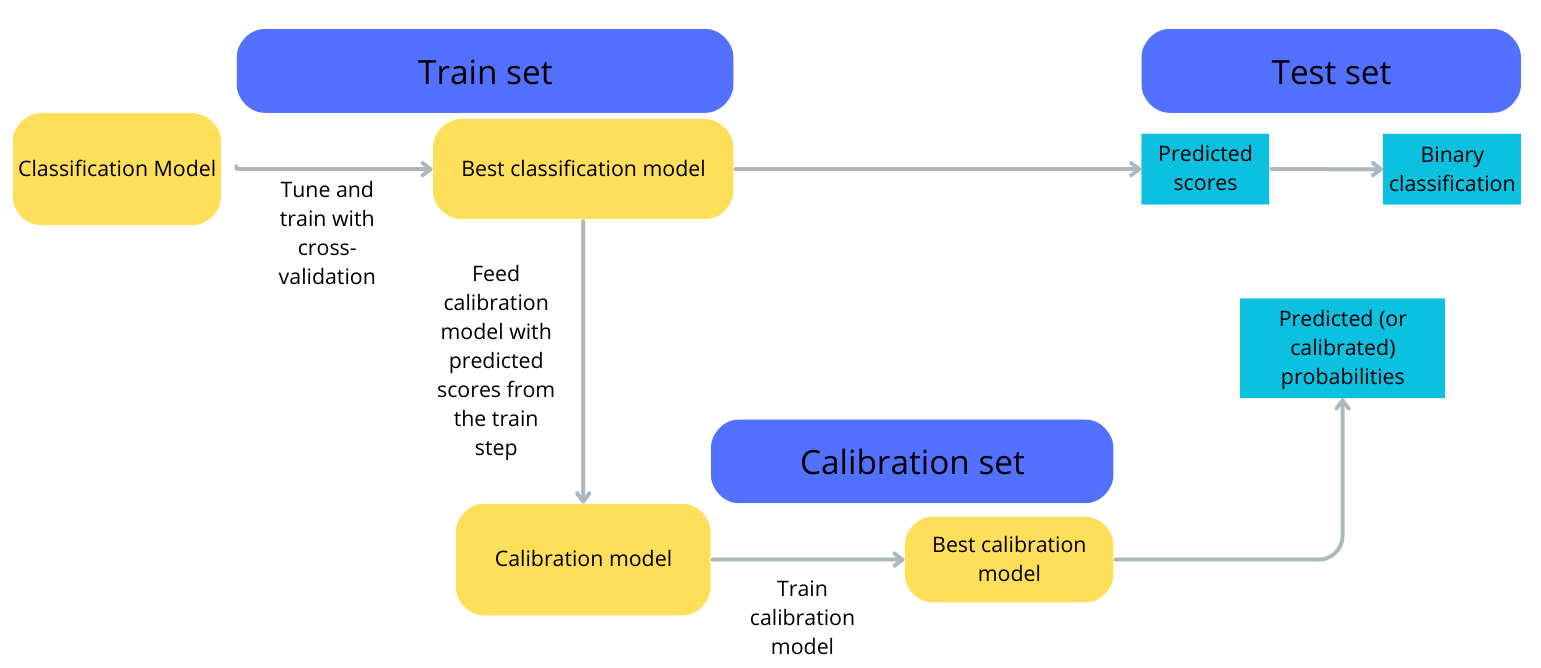
\includegraphics[width=1\textwidth]{Methodology.png}\\
    \caption{Training, calibration and testing methodology}
    \label{fig:Methodogoly}
\end{figure}
\FloatBarrier



\newpage
\section{Results}

The \autoref{tab:List of models} lists the results of the models. For each of them, the F1-Score, recall and precision have been calculated with their optimal classification threshold.

\paragraph{Classification model}
Model 1, the logistic regression used as a benchmark, is the model with the lowest classification performance. This shows that the classification is quite complex and that it is therefore useful to use more advanced machine learning models.\\
Both ensemble models without path duration are quite efficient with a recall of 0,74 (model 2) and 0,73 (model 3), which means they didn't predict much mishandled bags as successful and F1-Score and Precision between 0,7 and 0,75. 
Moreover, we can see that adding path duration (with residuals) allows models to improve their metrics by about 0,1 point.
Optimization by random search of hyper-parameters, on the other hand, managed to improve the F1-score of the \acrshort{rf} by 0,03 points and of the \acrshort{xgboost} by 0,01, which is very low. \\
Both probability calibration methods do not improve model scores.  This was to be expected as because the aim of probability calibration is to transform predicted scores into probabilities rather than to better classify the data.\hfill \break

The \autoref{fig:Probability_distribution_Model 1} shows the distribution of predicted probabilities for logistic regression, which is the least efficient model.
On the other hand, the \autoref{fig:Probability distribution - Model 10} shows the predicted probability distribution for model 10. This is the model I consider to be the most successful and that I recommend for use in the \autoref{sec:Conclusion}. These graphs have been made with sample data, to see how the predicted probabilities are distributed, and where the thresholds are located. 
We can see in blue the successful bags and in red the mishandlded luggage. On the ordinate, we have the probabilities predicted by the model. 
The higher the dots, the higher the predicted probability of a mishandled. Ideally, blue dots should be very low, red dots very high. 
As can be seen, the logistic regression does not classify failed and successful bags well. However, our best model shows a much better separated distribution between mishandled and successful baggage. The predicted probability distributions of the other models are all available in the appendix

To better analyze model results, we can also analyze confusion matrices. 
The \autoref{fig:Confusion_matrix_Model 1} and \autoref{fig:Confusion_matrix_Model 10} shows the confusion matrix of the benchmark model and the more efficient one (\acrshort{rf} with isotonic regression). Once again, we can see that logistic regression doesn't classify mishanlded luggage very well. In fact, for every bag it predicts to be mishanlded, 1,756 actually fail, while 2,918 succeed. This represents too much confusion. With such a model, too many bags that should have been successful could be predicted as misses.  However, for model 10, for all the baggage it predicts to mishandled, 2,616 actually miss, while only 223 successful. Clearly, our best-performing model is able to classify mishandled baggage much better than the reference model, which classifies with too many errors. 
In the appendix, \autoref{fig:Probability_density_Model 1} to \autoref{fig:Probability_density_Model 11} shows the density of predicted mishandled bags versus the density of predicted successful bags. These plots have redundant information with predicted probability distribution, but show the estimated density of all points (and not only samples). 
\FloatBarrier
\begin{figure}
\begin{minipage}[c]{0.4\linewidth}
    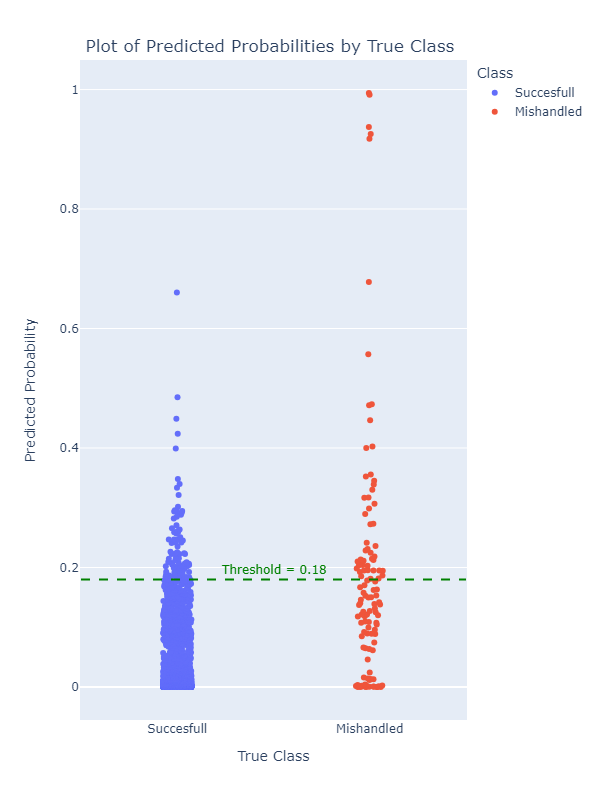
\includegraphics[width=1\textwidth]{Probability_distribution_Model 1.png}\\
    \caption{Probability distribution - Model 1}
    \label{fig:Probability_distribution_Model 1}
\end{minipage}%
\hfill
\begin{minipage}[c]{0.4\linewidth}
    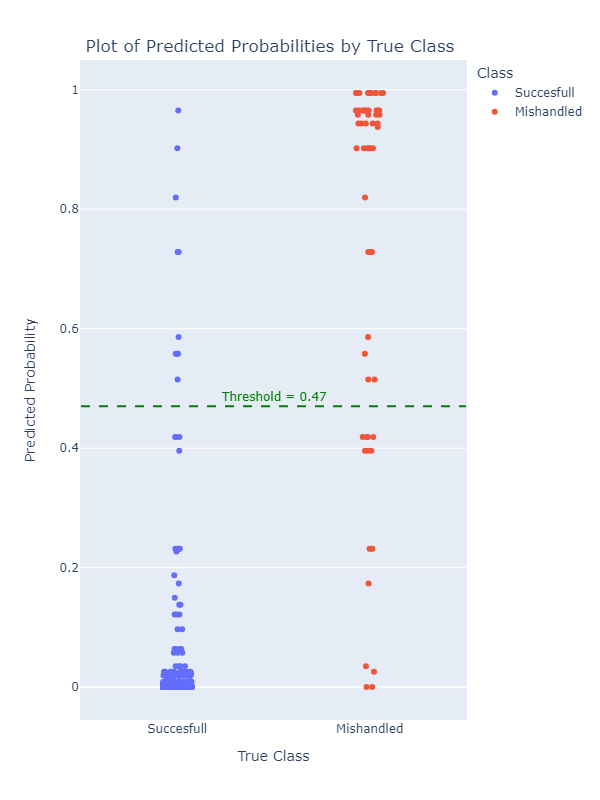
\includegraphics[width=1\textwidth]{Probability_distribution_Model 10.png}\\
    \caption{Probability distribution - Model 10}
    \label{fig:Probability distribution - Model 10}
\end{minipage}
\end{figure}
\FloatBarrier



\FloatBarrier
\begin{figure}
\begin{minipage}[c]{0.45\linewidth}
    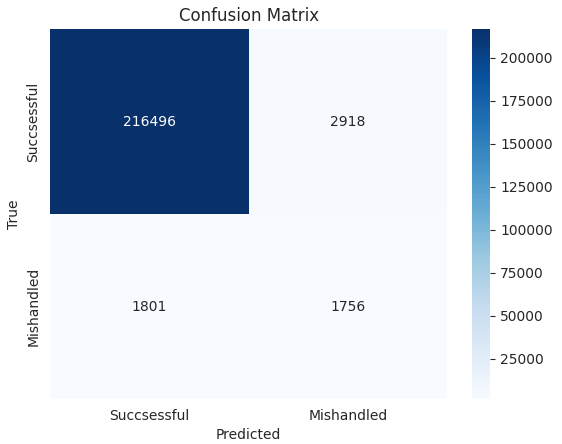
\includegraphics[width=1\textwidth]{Confusion_matrix_Model 1.png}\\
    \caption{Confusion matrix - Model 1}
    \label{fig:Confusion_matrix_Model 1}
\end{minipage}
\hfill
\begin{minipage}[c]{0.45\linewidth}
    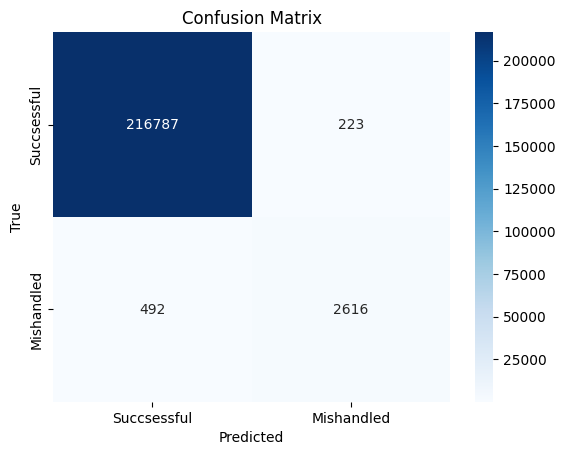
\includegraphics[width=1\textwidth]{Confusion_matrix_Model 10.png}\\
    \caption{Confusion matrix - Model 10}
    \label{fig:Confusion_matrix_Model 10}
\end{minipage}%
\end{figure}
\FloatBarrier






\paragraph{Probability calibration} We can see that the classification thresholds change after calibration, due to the fact that scores are transformed into probabilities, and the two are not equally distributed. To analyse and define the best probability calibration, we need to have a look at \autoref{fig:Probability calibration for xgboost} and \autoref{fig:Probability calibration for rf}. 
These two graphs compare the distribution of predicted scores (or probabilities) with the empirical proportions of mishandled baggage. Perfectly calibrated probabilities should follow the diagonal of the graph. In this case, we could say that on the bunch of bags where the predicted probability of mishandling is 70\%, the same proportion are actually mishandled. This would actually correspond to a probability, not a score. 
We can see that for XGBoost (blue line in the \autoref{fig:Probability calibration for xgboost}), the model tends to over-predict baggage with a score of 0,8. However, when the probabilities are calibrated by isotonic regression, they are under-predicted. Finally, platt-scaling does not improve but degrades score quality.
The \autoref{fig:Probability calibration for rf} shows that the probability calibration performed better for the \acrshort{rf} than the \acrshort{xgboost}. Indeed, the \acrshort{rf} without calibration tends to under-estimate scores between 0,4 and 0,95. However, the isotonic regression fits almost perfectly with the diagonal. With such a calibration, we can conclude that the \acrshort{rf} calibrated with an isotonic regression is the more accurate embedded model to calibrate and provide interpretable probabilities.


\FloatBarrier
\begin{figure}[h]
    \centering
    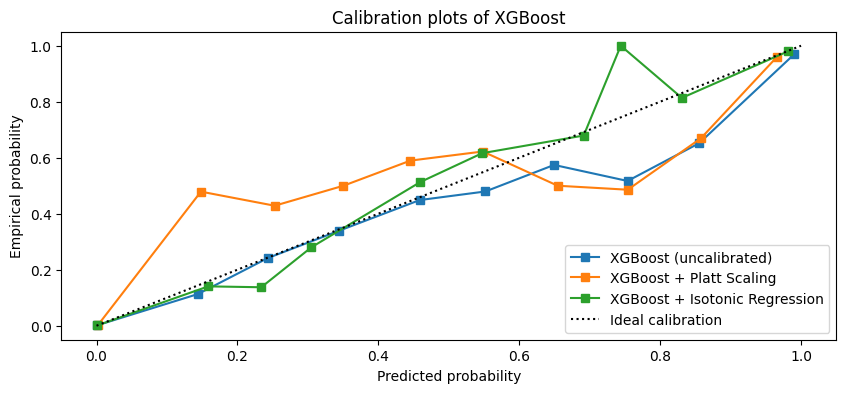
\includegraphics[width=0.7\textwidth]{Calibration_plot_XGBOOST.png}\\
    \caption{Probability calibration for \acrshort{xgboost}}
    \label{fig:Probability calibration for xgboost}
\end{figure}
\FloatBarrier

\FloatBarrier
\begin{figure}[h]
    \centering
    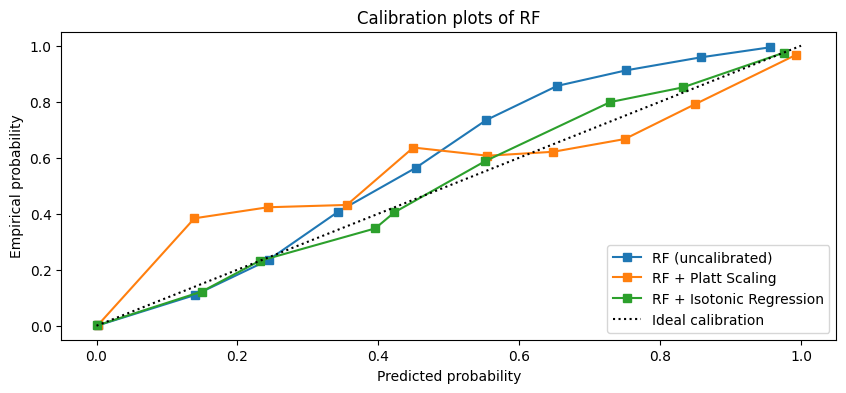
\includegraphics[width=0.7\textwidth]{Calibration_plot_RF.png}\\
    \caption{Probability calibration for \acrfull{rf}}
    \label{fig:Probability calibration for rf}
\end{figure}
\FloatBarrier


\paragraph{Feature importance in predictions}
Having predicted classifications and probabilities is pretty important and a good step forward in the aim to reduce mishandled baggage. However, understanding how models make their predictions could give us more insight to understand the reason baggage can be mishandled. As they are considered as black boxes, machine learning models are not easily interpretable. However, computing their shapley values (see \cite{Shapvalues}) allows to quantify the impact of features on model predictions. The \autoref{fig:Shap values} shows the shap values of the model 10. We can see that the most important variable is the number of minute before flight departure (\textit{input\_ICT\_BHS}). All of the red dots are on the left side of the figure, which can be interpreted as : when the baggage enters onto the \acrshort{bhs} with a large number of minute before flight departure, it is estimated more likely to be mishandled. In the other hand, if a baggage enters onto the BHS while its flight departure is planned in 5 minutes, it is more likely to be mishandled. This make sense and doesn't give much information to the handlers. However, this data is the most important in prediction. \hfill \break

The predicted path duration (or path duration with noise added) is the second most important data. This one is pretty important because if we actually manage to do an embedded model and predict path duration before the bag enters in the sorter, this shap value could warn handlers that there might have a problem in the sorter such that the path duration will be higher than planned.

\FloatBarrier
\begin{figure}[h]
    \centering
    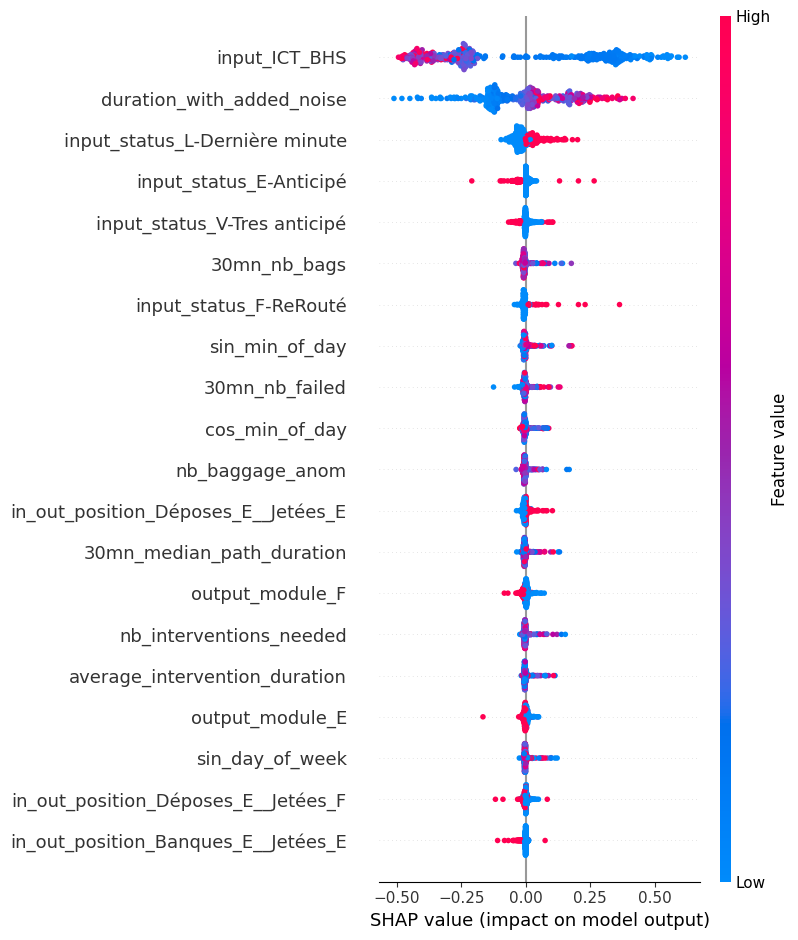
\includegraphics[width=0.7\textwidth]{shap values.png}\\
    \caption{Shap values of the model 10 (RF + Isotonic regression)}
    \label{fig:Shap values}
\end{figure}
\FloatBarrier

Moreover, this information can also be used in post operation analysis. If there was a day with a lot of mishandled baggage, \acrshort{adp} could use this model as to compute shap values and check out why and quantify the cause of mishandling. This could help in the allocation of responsibility between \acrshort{adp} and Air France\footnote{As Air France is in charge of baggage logistic outside the \acrshort{bhs}} for mishandled baggage. If a baggage is predicted mishandled due to a longer path duration predicted, this would mean \acrshort{adp} is responsible of the mishandling. On the other hand, if a baggage is missed because it has a short amount of time before flight departure, it means Air France injected it too late and they might be responsible. About the other features, we see that they all have a lower impact. Still, those impact are not insignificant. \hfill \break

Finally, I computed the individual shap values for three mishandled baggage. The \autoref{fig:Shap values of a random mishandled baggage (1)} is pretty interesting, as wee see that he model predicted the baggage to be mishandled, not only because of its path duration or the number of minute before flight departure. The probability of being mishandled increased thanks to a lot of variables. In this case, it would be interesting to analyse the baggage path and see what was the reason of its mishandling. \hfill \break

The \autoref{fig:Shap values of a random mishandled baggage (2)} shows that the model predicted a successful baggage aleven thought it was mishandled. The number of minute before flight departure have reduced the predicted probability to be mishandled, this most likely means that the baggage wasn't injected onto the \acrshort{bhs} too late. In contrast, the predicted path duration slightly increased the predicted probability. According to those values, we could conclude that something went wrong during the journey in the \acrshort{bhs}. \hfill \break

Finally, the \autoref{fig:Shap values of a random mishandled baggage (3)} shows that the model clearly predicted the baggage to be mishandled because it had not enough time before flight departure. With such values, we could conclude that it arrived too late and the \acrshort{bhs} did not mishandled it.

\section*{Conclusion}
\addcontentsline{toc}{section}{Conclusion}
\label{sec:Conclusion}


Based on the results, I would suggest to use the model 10 (\acrshort{rf} calibrated by isotonic regression), for both  classifying and predicting probabilities. Computing the shap values in real time could also help handlers to take decisions. Moreover, those values can also be used in post operations analysis to help the analyst to understand the reasons of a mishandling.

Furthermore, all of my models were trained and tested for three months. Adding the variable "\textit{date of month}" and training the model on a longer period could make it learn more seasonal variations and cyclical patterns.

Testing the models under conditions of high logistical disruption (or high rate of mishandled bags) could be a good experimentation. This could provide rigorous stress-test, allowing to observe how the model behaves under complicated circumstances. If the model performance remains stable, it would mean it is confident even when there are a lot of perturbations in the logistic process.

Further investigations should be made on the use of path duration. If a predictive model on this variable is finished, I would suggest to compare features used in both models and to make sure they don't have the same. If embedding of both models ends-up to be impossible, the models 2 and 3 (models not using predicted path duration) could be calibrated. They have a lower performance as they don't use the path duration, but still can be improved and used. 

The use of over or under sampling could be an idea to increase the models performances. However, I didn't use those methods as my scores were higher than expected without sampling. By using such methods, we would be more likely to over fit our models, so they should be applied rigorously.

\newpage
\section*{Appendix}
\addcontentsline{toc}{section}{Appendix}




\FloatBarrier
\begin{figure}[h]
    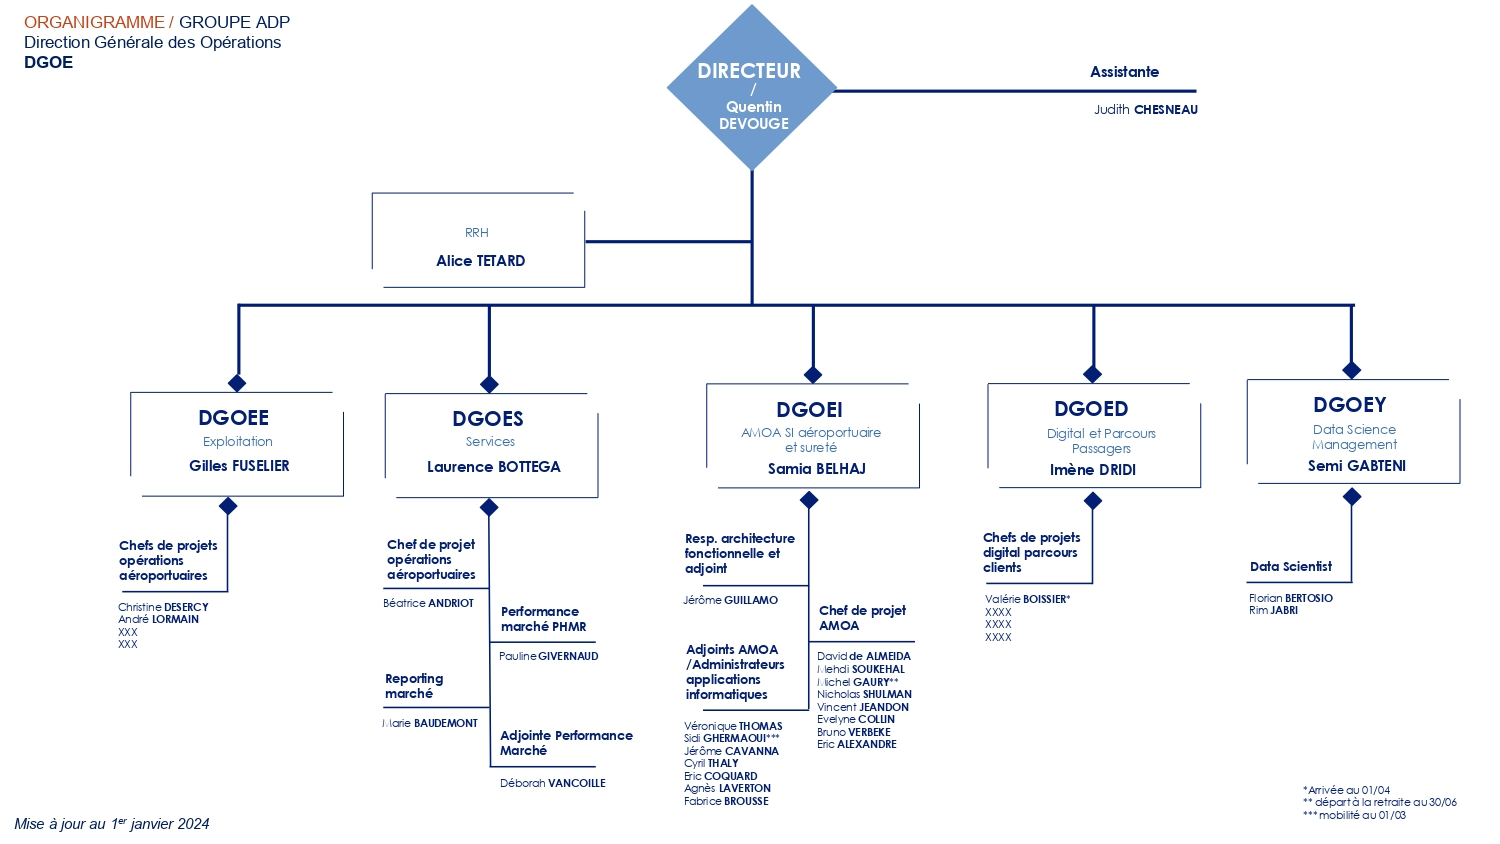
\includegraphics[width=1\textwidth]{organigramme_DGO.jpg}\\
    \caption{\acrshort{dgo} organization chart}
    \label{fig:DGO organization chart}
\end{figure}
\FloatBarrier



\FloatBarrier
\begin{table}[ht]
\centering
\caption{List of models}
\label{tab:List of models}
\renewcommand{\arraystretch}{3}
\begin{small}
\begin{tabularx}{\textwidth}{|c|X|X|c|c|c|c|}
\hline
\textbf{ID} & \textbf{Name} & \textbf{Description} & \textbf{Threshold} & \textbf{F1-Score} & \textbf{Recall} & \textbf{Precision} \\ \hline
1 & Logistic regression & Main features & 0.18 & 0.43 & 0.49 & 0.38  \\ \hline
2 & RF & Main features & 0.33 & 0.76 & 0.74 & 0.78  \\ \hline
3 & XGBoost & Main features & 0.7 & 0.74 & 0.73 & 0.75 \\ \hline
4 & RF & Path duration with noise added & 0.34 & 0.85 & 0.85 & 0.9  \\ \hline
5 & XGBoost & Path duration with noise added & 0.61 & 0.88 & 0.87 & 0.9  \\ \hline
6 & RF & Random search optimization & 0.37 & 0.88 & 0.85 & 0.9  \\ \hline
7 & XGBoost & Random search optimization & 0.45 & 0.89 & 0.87 & 0.9  \\ \hline
8 & RF + Platt scaling & Platt scaling for probability calibration & 0.39 & 0.88 & 0.84 & 0.93 \\ \hline
9 & XGBoost + Platt scaling & Platt scaling for probability calibration & 0.13 & 0.88 & 0.87 & 0.9  \\ \hline
10 & RF + Isotonic regression & Isotonic regression for probability calibration & 0.47 & 0.88 & 0.84 & 0.92  \\ \hline
11 & XGBoost + Isotonic regression & Isotonic regression for probability calibration & 0.35 & 0.89 & 0.88 & 0.9 \\ \hline
\end{tabularx}
\end{small}
\end{table}
\FloatBarrier


\begin{figure}
\begin{minipage}[c]{0.45\linewidth}
    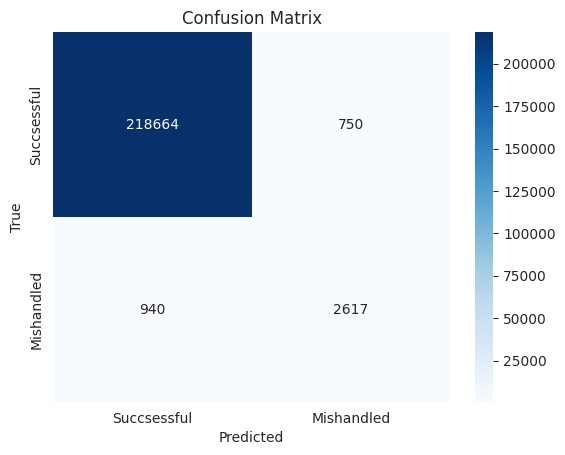
\includegraphics[width=1\textwidth]{Confusion_matrix_Model 2.jpg}\\
    \caption{Confusion matrix - Model 2}
\end{minipage}%
\hfill
\begin{minipage}[c]{0.45\linewidth}
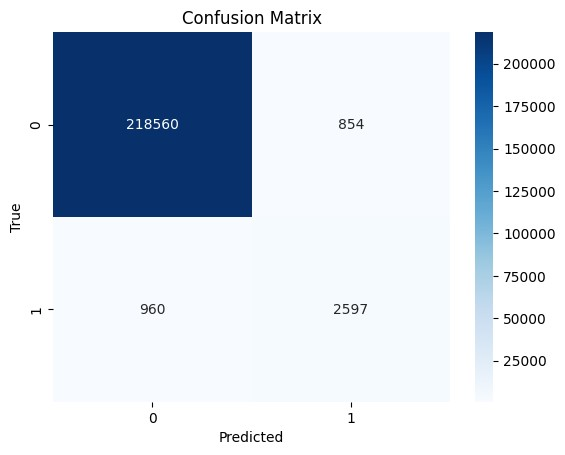
\includegraphics[width=1\textwidth]{Confusion_matrix_Model 3.jpg}\\
\caption{Confusion matrix - Model 3}
\end{minipage}
\break
\begin{minipage}[c]{0.45\linewidth}
    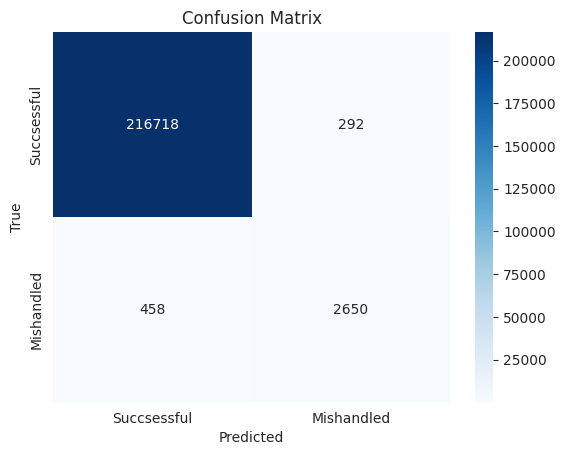
\includegraphics[width=1\textwidth]{Confusion_matrix_Model 4.png}\\
    \caption{Confusion matrix - Model 4}
\end{minipage}%
\hfill
\begin{minipage}[c]{0.45\linewidth}
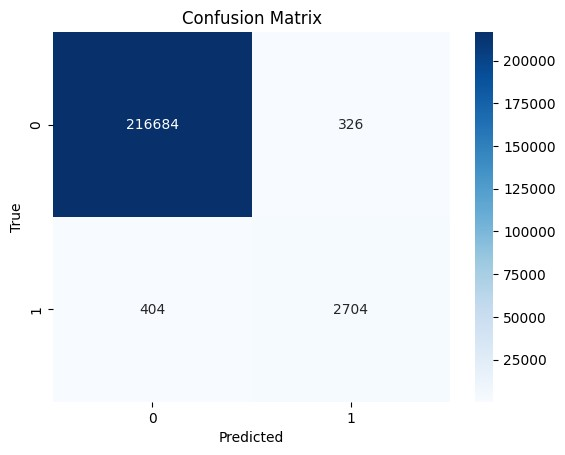
\includegraphics[width=1\textwidth]{Confusion_matrix_Model 5.jpg}\\
\caption{Confusion matrix - Model 5}
\end{minipage}
\break
\begin{minipage}[c]{0.45\linewidth}
    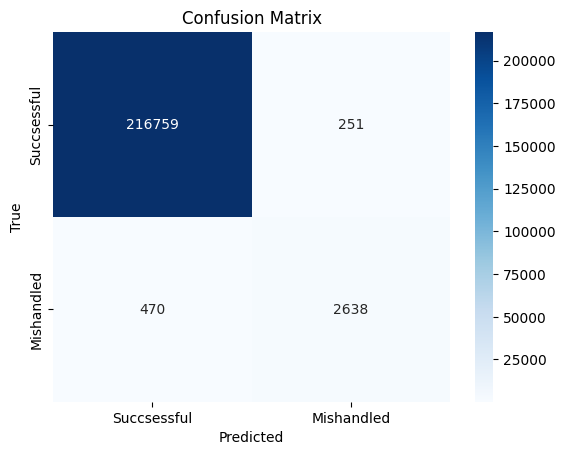
\includegraphics[width=1\textwidth]{Confusion_matrix_Model 6.png}\\
    \caption{Confusion matrix - Model 6}
\end{minipage}%
\hfill
\begin{minipage}[c]{0.45\linewidth}
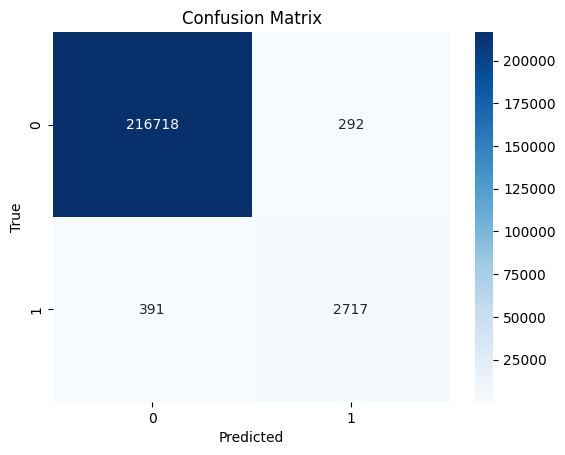
\includegraphics[width=1\textwidth]{Confusion_matrix_Model 7.png}\\
\caption{Confusion matrix - Model 7}
\end{minipage}
\end{figure}

\begin{figure}
\begin{minipage}[c]{0.45\linewidth}
    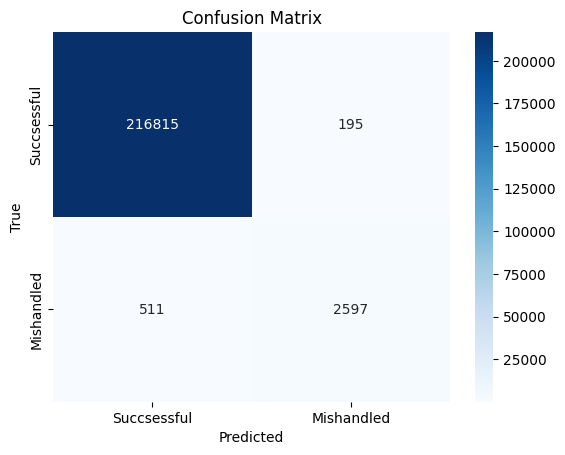
\includegraphics[width=1\textwidth]{Confusion_matrix_Model 8.png}\\
    \caption{Confusion matrix - Model 8}
\end{minipage}%
\hfill
\begin{minipage}[c]{0.45\linewidth}
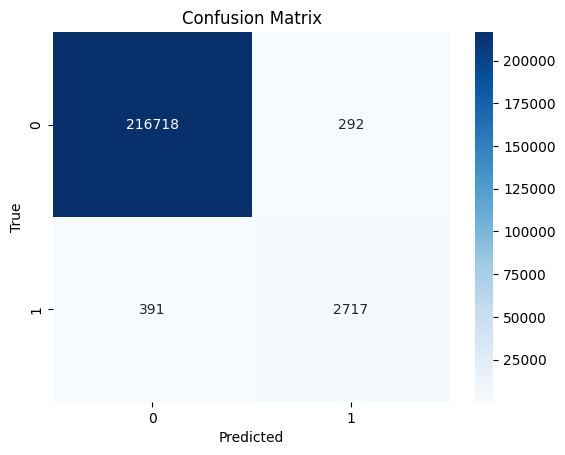
\includegraphics[width=1\textwidth]{Confusion_matrix_Model 9.png}\\
\caption{Confusion matrix - Model 9}
\end{minipage}
\break
\begin{minipage}[c]{0.45\linewidth}
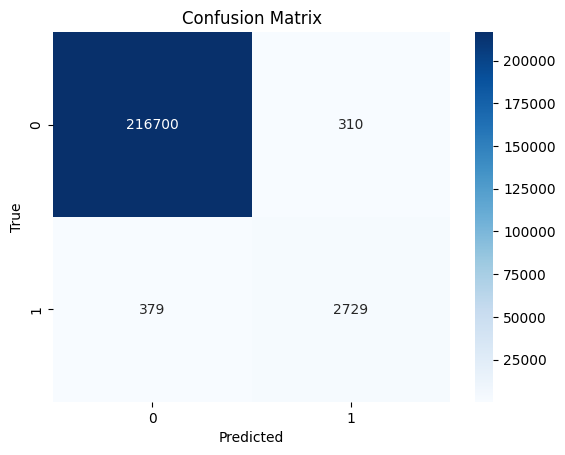
\includegraphics[width=1\textwidth]{Confusion_matrix_Model 11.png}\\
\caption{Confusion matrix - Model 11}
\end{minipage}
\begin{minipage}[c]{0.45\linewidth}

\end{minipage}
\end{figure}


\FloatBarrier
\begin{figure}
\begin{minipage}[c]{0.4\linewidth}
    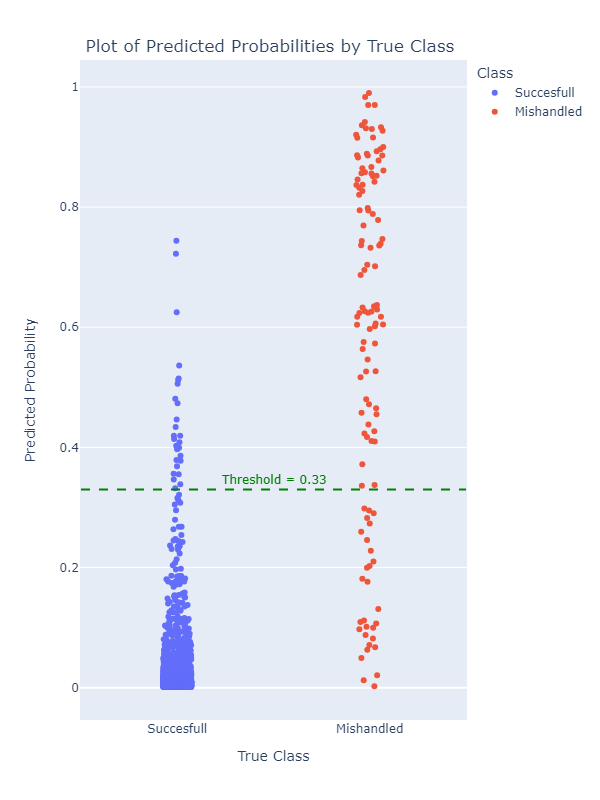
\includegraphics[width=1\textwidth]{Probability_distribution_Model 2.png}\\
    \caption{Probability distribution - Model 2}
\end{minipage}%
\hfill
\begin{minipage}[c]{0.4\linewidth}
    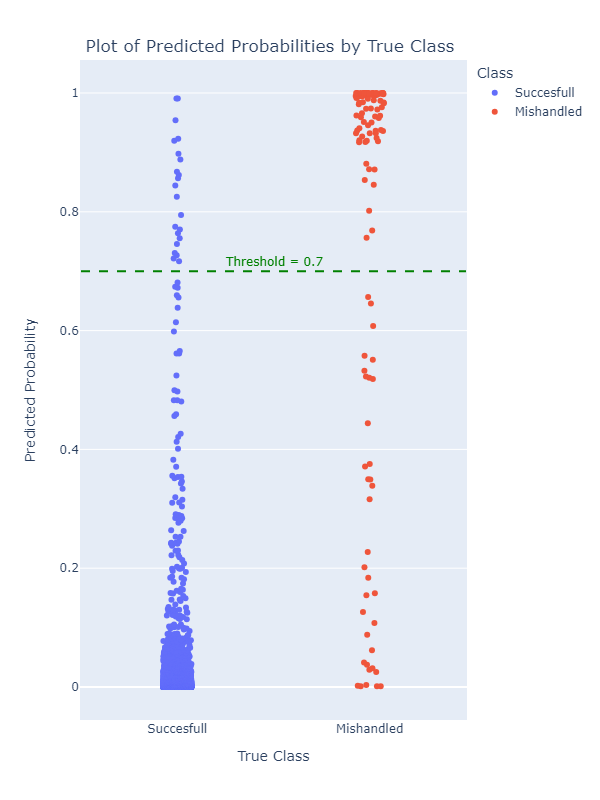
\includegraphics[width=1\textwidth]{Probability_distribution_Model 3.png}\\
    \caption{Probability distribution - Model 3}
\end{minipage}
\end{figure}

\begin{figure}
\begin{minipage}[c]{0.4\linewidth}
    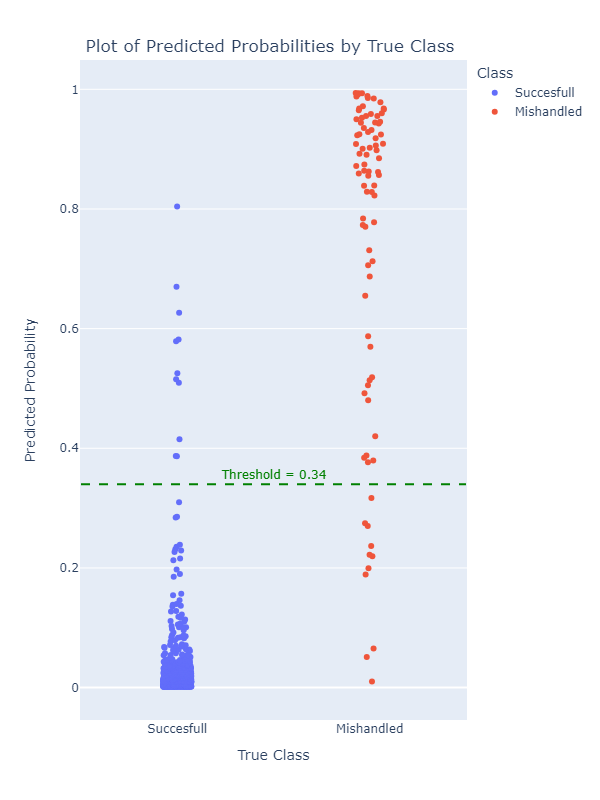
\includegraphics[width=1\textwidth]{Probability_distribution_Model 4.png}\\
    \caption{Probability distribution - Model 4}
\end{minipage}%
\hfill
\begin{minipage}[c]{0.4\linewidth}
    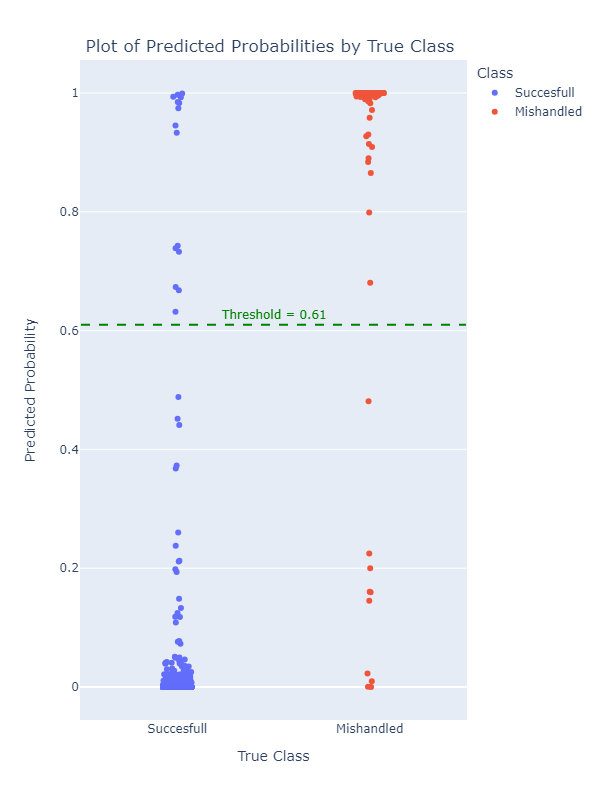
\includegraphics[width=1\textwidth]{Probability_distribution_Model 5.png}\\
    \caption{Probability distribution - Model 5}
\end{minipage}
\end{figure}

\begin{figure}
\begin{minipage}[c]{0.4\linewidth}
    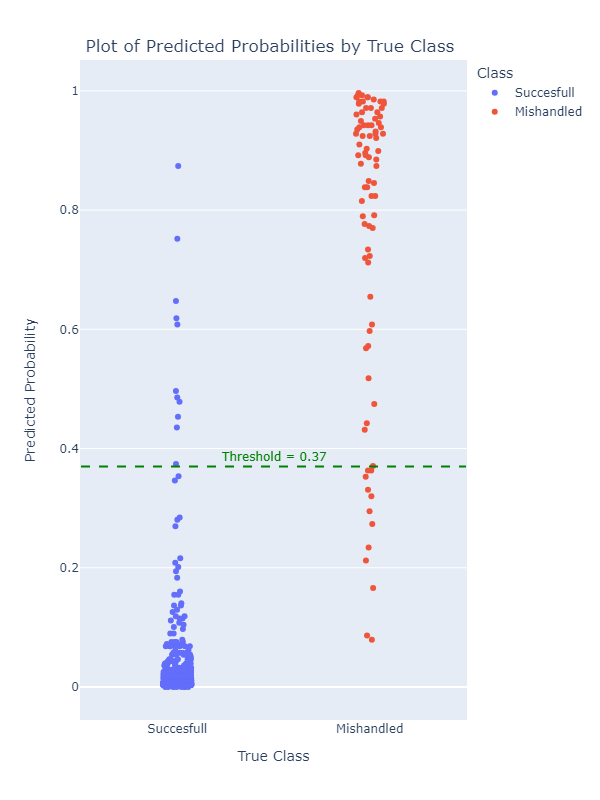
\includegraphics[width=1\textwidth]{Probability_distribution_Model 6.png}\\
    \caption{Probability distribution - Model 6}
\end{minipage}%
\hfill
\begin{minipage}[c]{0.4\linewidth}
    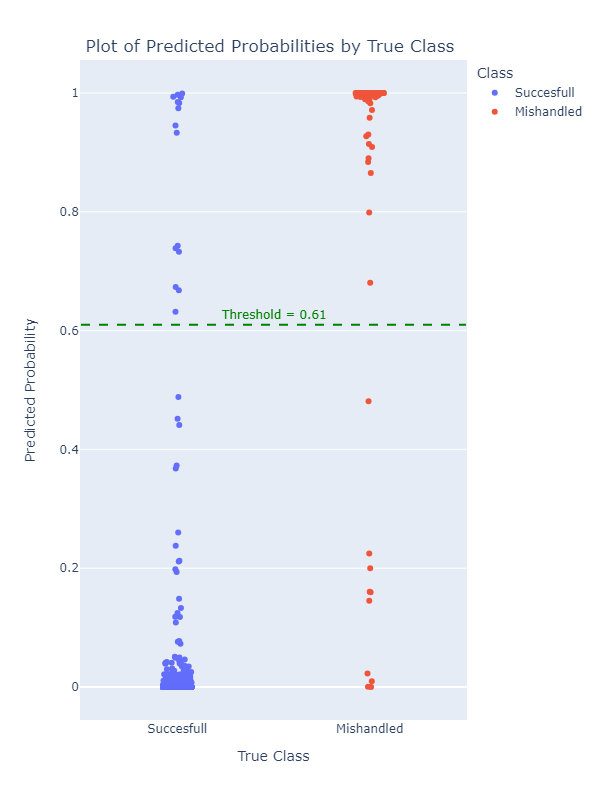
\includegraphics[width=1\textwidth]{Probability_distribution_Model 7.png}\\
    \caption{Probability distribution - Model 7}
\end{minipage}
\end{figure}

\begin{figure}
\begin{minipage}[c]{0.4\linewidth}
    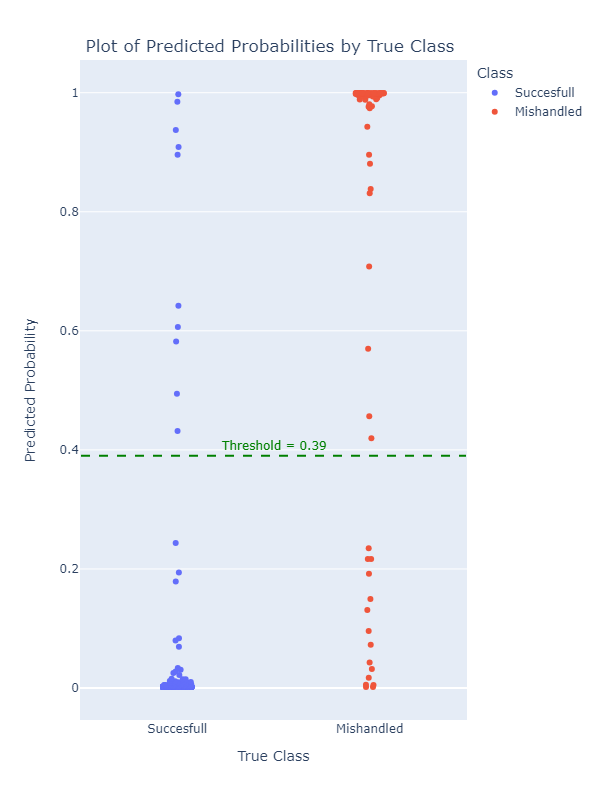
\includegraphics[width=1\textwidth]{Probability_distribution_Model 8.png}\\
    \caption{Probability distribution - Model 8}
\end{minipage}%
\hfill
\begin{minipage}[c]{0.4\linewidth}
    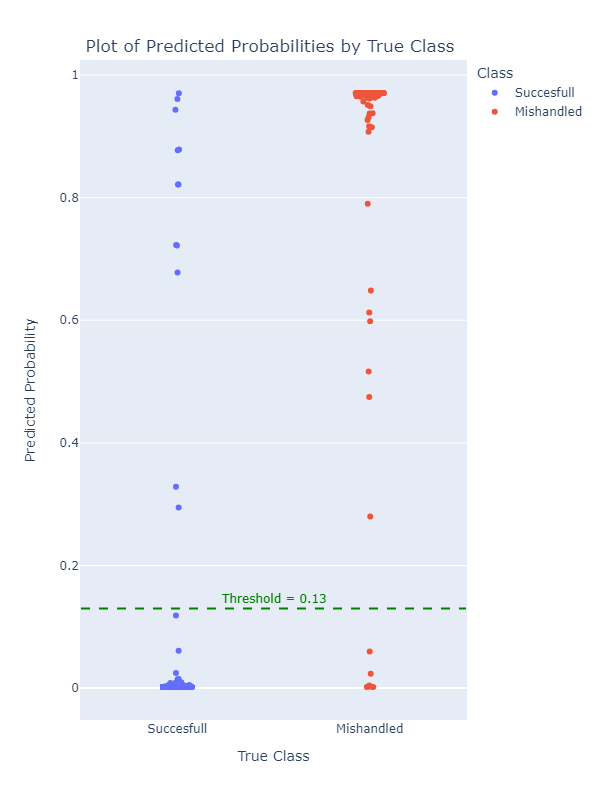
\includegraphics[width=1\textwidth]{Probability_distribution_Model 9.png}\\
    \caption{Probability distribution - Model 9}
\end{minipage}
\end{figure}

\begin{figure}
\begin{minipage}[c]{0.4\linewidth}
    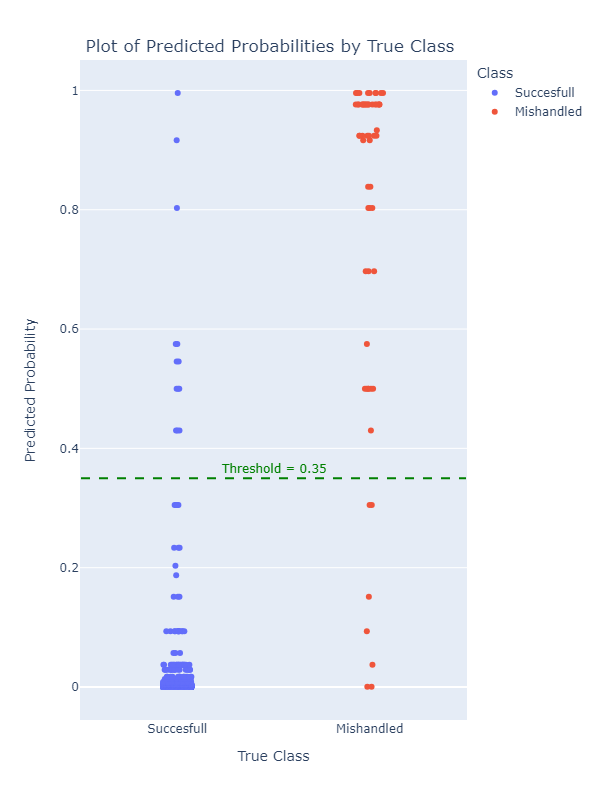
\includegraphics[width=1\textwidth]{Probability_distribution_Model 11.png}\\
    \caption{Probability distribution - Model 11}
\end{minipage}
\hfill
\begin{minipage}[c]{0.4\linewidth}
\end{minipage}%
\end{figure}
\FloatBarrier




\FloatBarrier
\begin{figure}
\begin{minipage}[c]{0.5\linewidth}
    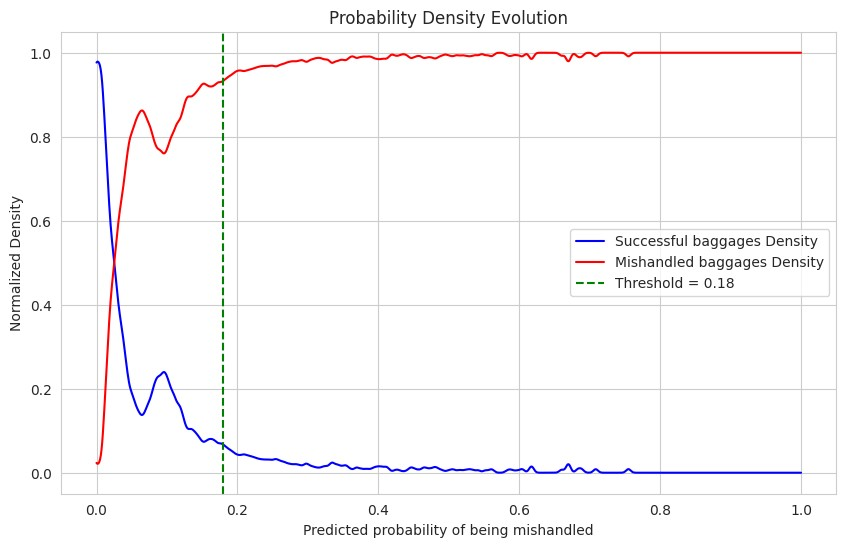
\includegraphics[width=1\textwidth]{Probability_density_Model 1.jpg}\\
    \caption{Probability density - Model 1}
    \label{fig:Probability_density_Model 1}
\end{minipage}
\hfill
\begin{minipage}[c]{0.5\linewidth}
    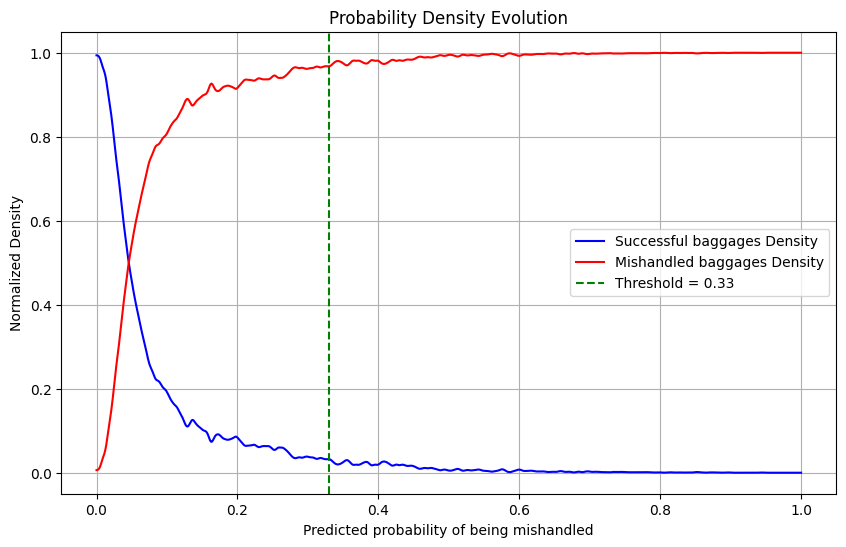
\includegraphics[width=1\textwidth]{Probability_density_Model 2.png}\\
    \caption{Probability density - Model 2}
\end{minipage}%
\break
\begin{minipage}[c]{0.5\linewidth}
    \includegraphics[width=1\textwidth]{Probability_density_Model 3.jpg}\\
    \caption{Probability density - Model 3}
\end{minipage}
\hfill
\begin{minipage}[c]{0.5\linewidth}
    \includegraphics[width=1\textwidth]{Probability_density_Model 4.png}\\
    \caption{Probability density - Model 4}
\end{minipage}
\break
\begin{minipage}[c]{0.5\linewidth}
    \includegraphics[width=1\textwidth]{Probability_density_Model 5.jpg}\\
    \caption{Probability density - Model 5}
\end{minipage}
\hfill
\begin{minipage}[c]{0.5\linewidth}
    \includegraphics[width=1\textwidth]{Probability_density_Model 6.png}\\
    \caption{Probability density - Model 6}
\end{minipage}%
\end{figure}
\begin{figure}
\begin{minipage}[c]{0.5\linewidth}
    \includegraphics[width=1\textwidth]{Probability_density_Model 7.png}\\
    \caption{Probability density - Model 7}
\end{minipage}
\hfill
\begin{minipage}[c]{0.5\linewidth}
    \includegraphics[width=1\textwidth]{Probability_density_Model 8.png}\\
    \caption{Probability density - Model 8}
\end{minipage}%
\break
\begin{minipage}[c]{0.5\linewidth}
    \includegraphics[width=1\textwidth]{Probability_density_Model 9.png}\\
    \caption{Probability density - Model 9}
\end{minipage}
\hfill
\begin{minipage}[c]{0.5\linewidth}
    \includegraphics[width=1\textwidth]{Probability_density_Model 10.png}\\
    \caption{Probability density - Model 10}
\end{minipage}%
\break
\begin{minipage}[c]{0.5\linewidth}
    \includegraphics[width=1\textwidth]{Probability_density_Model 11.png}\\
    \caption{Probability density - Model 11}
    \label{fig:Probability_density_Model 11}
\end{minipage}
\hfill
\begin{minipage}[c]{0.5\linewidth}
\end{minipage}%
\end{figure}
\FloatBarrier







\begin{figure}[h]
    \centering
    \includegraphics[width=0.9\textwidth]{cyclical encoding.png}\\
    \caption{Cyclical encoding of days and minutes}
    \label{fig:Cyclical encoding of days and minutes}
\end{figure}
\FloatBarrier

\FloatBarrier
\begin{figure}[ht]
  \centering
  \begin{subfigure}{0.48\textwidth}
    \includegraphics[width=\linewidth]{percentage of failed per module.png}
    \caption{Percentage of mishandled bags according to input and output modules}
    \label{fig:Percentage of mishandled bags according to input and output modules}
  \end{subfigure}
  \hfill
  \begin{subfigure}{0.48\textwidth}
    \includegraphics[width=\linewidth]{number of bags per module.png}
    \caption{Number of bags according to input and output modules}
    \label{fig:Number of bags according to input and output modules}
  \end{subfigure}
  \caption{Mishandled bags according to modules}
  \label{fig:Mishandled bags according to modules}
\end{figure}


\begin{figure}
\begin{minipage}[c]{0.5\linewidth}
    \includegraphics[width=1\textwidth]{shap values 1.png}
    \caption{Shap values of a random mishandled baggage (1)}
    \label{fig:Shap values of a random mishandled baggage (1)}
\end{minipage}
\hfill
\begin{minipage}[c]{0.5\linewidth}
    \includegraphics[width=1\textwidth]{shap values 2.png}
    \caption{Shap values of a random mishandled baggage (2)}
    \label{fig:Shap values of a random mishandled baggage (2)}
\end{minipage}
\break
\begin{minipage}[c]{0.5\linewidth}
    \includegraphics[width=1\textwidth]{shap values 3.png}
    \caption{Shap values of a random mishandled baggage (3)}
    \label{fig:Shap values of a random mishandled baggage (3)}
\end{minipage}
\hfill
\begin{minipage}[c]{0.5\linewidth}
\end{minipage}%
\end{figure}






\newpage
\FloatBarrier
\printglossaries
\FloatBarrier


\newpage
\printbibliography




\end{document}
